\documentclass[sigconf,review,anonymous]{acmart}
\usepackage{booktabs}
\usepackage{array}
\setlength{\emergencystretch}{2.5em}
\setcopyright{none}
\settopmatter{printacmref=false}
\renewcommand\footnotetextcopyrightpermission[1]{}

\newtheorem{proposition}{Proposition}

\newcommand{\Rcomm}{R_{\text{comm}}}
\newcommand{\Rext}{R_{\text{ext}}}
\newcommand{\Rtotal}{R_{\text{total}}}
\newcommand{\VL}{V_L}
\newcommand{\AlphaRL}{\alpha_{\text{RL}}}
\newcommand{\AlphaRSA}{\alpha_{\text{RSA}}}
\newcommand{\Ltheta}{L_\theta}

\title{Which Listener? Counterfactual Anchoring for Pragmatic Legibility Rewards in Multi-Agent Reinforcement Learning}

\author{Anonymous Author(s)}
\affiliation{\institution{Anonymous Institution}\city{}\country{}}

\begin{document}

\begin{abstract}
\setlength{\emergencystretch}{2em}%
Cooperative RL agents often fail because their intentions are illegible to partners, not because they act poorly. We study an intrinsic reward for legibility, imported from the Rational Speech Act (RSA) model of pragmatics via its structural correspondence with maximum-entropy RL: a listener's log-posterior over an agent's private state given its behavior, computed offline at no execution-time cost; its decisive design choice is which literal listener $L_0$ anchors it. Any listener makes the reward a variational bound on intent--behavior mutual information, and one that decodes confidently supplies little shaping gradient. On \emph{scout-support}, whose oracle-gap criterion certifies communication has task value, hand-crafted motion-grounded listeners close $61$--$82\%$ of the oracle premium (Welch $t\ge4$; the $82\%$ endpoint, $t{=}3.98$, survives Bonferroni). Learned listeners fail by succeeding: trained to convergence they decode any behavior, saturate and shape nothing, and bounding them to the partner's viewpoint does not help; RSA recursion recovers $27\%$ (held-out confirmation). The resolution is the \emph{inverse-planning listener}, which Bayes-inverts a frozen non-communicative baseline and closes $55$--$70\%$ ($t\ge3.6$), the same band as the best hand-crafted listener with no task-specific geometry. An ablation isolates why: two listeners read off the \emph{same} frozen policy diverge completely---$69\%$ closure versus none ($3.2\%$, n.s.)---depending only on whether the listener is \emph{queried counterfactually} across candidate meanings or \emph{fitted} to that policy's rollouts. Hence \emph{counterfactual anchoring}: score behavior against what a competent reference would do under each candidate meaning, not against a listener fitted to the speaker's own. We map where the effect holds and extend the reward to continuous meaning spaces and to an agent's own bottlenecked decision latent, whose behavioral readability it raises without altering its content (suggestive tier). Training $3\times$ past the evaluation budget then separates what the reward buys: the oracle premium is largely a learning-speed transient (settling $1.8\times$ smaller) and task capture declines with it ($72\%$ to $36\%$), while the readability gap the reward creates \emph{widens} in the paying listener's vocabulary---the no-incentive oracle drifting below baseline---and the signal is grounded rather than conventional: decoders fitted to one seed read every other seed, and a frozen-policy reader recovers $90$--$97\%$ of what any fitted one finds. The dissociation survives the asymptote---every grounded anchor keeps a converged gain, the co-adapting listener keeps none---and what the reward durably purchases is legible behavior.
\end{abstract}

\begin{CCSXML}
<ccs2012>
<concept>
<concept_id>10010147.10010178.10010219</concept_id>
<concept_desc>Computing methodologies~Multi-agent systems</concept_desc>
<concept_significance>500</concept_significance>
</concept>
</ccs2012>
\end{CCSXML}
\ccsdesc[500]{Computing methodologies~Multi-agent systems}
\keywords{multi-agent reinforcement learning; legibility; intrinsic motivation; computational pragmatics; implicit communication}

\maketitle

\section{Introduction}
\label{sec:intro}

In cooperative multi-agent reinforcement learning (MARL), success depends not only on acting well but on being \emph{understood}: an agent rushing along an ambiguous path can make a partner abandon a target it never meant to claim, while a slightly suboptimal path that singles that target out enables coordination. This is legibility \cite{dragan2013legibility}, and agents optimized for task reward alone have no incentive to possess it.

We study an intrinsic reward $\Rcomm$ for communicative clarity, modelling an observer that reasons pragmatically about \emph{why} the agent chose its action over the alternatives \cite{goodman2016pragmatic}. Any such observer rests on a \emph{literal listener} $L_0$: the common ground fixing how behavior is read absent pragmatic reasoning. This choice decides whether legibility rewards help or hurt, and it fails at both extremes: a hand-crafted $L_0$ can be misaligned with what the policy can express, buying costly signaling no observer decodes, while a learned $L_0$ guarantees decodability but, trained to convergence, decodes \emph{everything} and demands nothing, its reward saturating as a gradient-saturation bound formalizes. Mapping the productive region between is this paper's empirical core.

\textbf{(1) A pragmatic derivation, with theory locating the listener space.} Max-Ent RL and RSA are both softmax choice models, a correspondence that imports the RSA listener value as an offline, CTDE-compatible intrinsic reward (purely communicative models such as CRSA \cite{estienne2025collaborative} occupy the myopic corner of the same objective). \emph{Any} listener makes the expected reward a variational lower bound on $I(M;S,A)$, which ML training merely tightens \cite{strouse2018learning,eysenbach2019diversity}; a \emph{gradient-saturation} bound shows a confident decoder shapes correspondingly little---the tightest bound can be the worst reward---and a \emph{vocabulary-restriction} proposition shows a listener factoring through reader-computable statistics pays only for codes the reader can extract. Both follow from how the listener is built rather than being imposed on it: a listener \emph{fitted} to the speaker's behavior decodes through context the reader never sees, whereas one \emph{queried counterfactually} across candidate meanings moves only with what the action discriminates. We call this \emph{counterfactual anchoring}. \textbf{(2) An evaluation protocol.} The \emph{oracle-gap} criterion adapts the Dec-POMDP value-of-communication gap \cite{pynadath2002communicative,goldman2003optimizing,oliehoek2016concise} into an admission gate for deep-MARL benchmarks; \emph{scout-support} makes task-optimal motion uninformative exactly when information is needed; a blind-partner control separates communication from shaping; and a documented pre-convergence hazard shows why converged budgets are non-negotiable for co-adaptive measures---and, at $3\times$ that budget, that orderings stabilize long before magnitudes: the premium itself is largely a learning-speed transient whose durable residue is legibility (Sec.~\ref{ssec:results_dynamics}). \textbf{(3) An empirical map and a constructive recipe.} Hand-crafted motion-grounded listeners close $61$--$82\%$ of the premium (Welch $t\ge4$, frozen hyperparameters, three variants); co-adapting learned listeners saturate and shape nothing even under input and window bounds, RSA recursion restoring a quarter; and the \emph{inverse-planning listener}---a Boltzmann observer self-instantiated from a frozen non-communicative baseline---closes $55$--$70\%$ ($t\ge3.6$), the same band as the best hand-crafted listener, with no task-specific geometry. Premium-vs-cost sweeps yield a proportionality regularity with characterized failure modes; on a continuous meaning space the literal listener stays inert and the recursion's advantage never reverses sign while premiums shrink. \textbf{(4) Legible latents: meanings discovered, not specified.} Routing private observation through a variational bottleneck and aiming the particle recursion at the agent's \emph{own} decision latent yields, to our knowledge, the first oracle-certified premium for exposing a \emph{learned} latent the designer never specified---task pressure selects its content, decoy-verified---while the reward raises its behavioral readability ($I(Z;\text{beh})$ up, $t{\approx}4.6$) and leaves content and private budget unchanged. Premium and protocol are certified; closures here are suggestive-tier.

\section{Related Work}
\label{sec:related}

\textbf{Legibility and observer-aware rewards.} Legibility inverts goal inference \cite{ziebart2008maximum,baker2017rational,ramirez2010plan}: the actor shapes behavior so an observer's inference succeeds. Formalized for robot motion \cite{dragan2013legibility}, it extends to sequential tasks (including goal-posterior rewards from Boltzmann-inverted per-goal optimal values \cite{faria2024guess}, the construction our inverse-planning listener ports to deep MARL), observer-aware MDPs \cite{miura2021unifying,miura2024observer}, and multiagent RL via belief-gain shaping \cite{liu2025active}. Observer models have served as in-RL reward signals before: in policy search and shaping against human observers \cite{busch2017learning,bied2020integrating}, as supervised models \cite{wallkotter2022slotv}, as log-posterior regularization on frozen pretrained Q-functions \cite{persiani2022policy}, and as Boltzmann-observer self-rewards in teacher--learner pedagogy \cite{caselles2022pragmatically}; goal-recognition design modifies \emph{environments} toward the same objective \cite{keren2014goal}. Bayesian pedagogy reaches the mechanism from teaching \cite{ho2016showing,fisac2017pragmatic}, cooperative inverse RL supplies its game-theoretic form and pedagogic equilibria \cite{hadfieldmenell2016cooperative}, and reward-rational choice unifies behavior-as-evidence \cite{jeon2020reward}; Milli and Dragan ask, on the learner's side, whether to assume a literal or pedagogic partner \cite{milli2019literal}---the model-choice question we pose on the reward side. Our additions are the Max-Ent/RSA derivation, the first \emph{systematic} listener-choice study in deep MARL under a certified-premium protocol, and the boundary map: the listener constructions have precedents, which we measure head-to-head rather than re-invent.

\textbf{Intrinsic rewards for coordination.} Closest to $\Rcomm$ is Tian et al.'s auxiliary reward~\cite{tian2020implicit}, paying an agent for its partner's correct belief about action-transmitted private information; fixing the audience to the partner's own inference network is one point in the listener space we sweep, evaluated head-to-head in Sec.~\ref{ssec:results_scout} alongside a variational instantiation of the conditional-information regularizer $I(A;G|S)$ of Strouse et al.~\cite{strouse2018learning}. Social influence \cite{jaques2019social} rewards \emph{compelling} a partner's reaction; $\Rcomm$ rewards transmission, leaving teammates free to exploit or ignore the revealed intention. In Hanabi, the Bayesian action decoder's public belief lets agents \emph{act informatively} because they know they will be decoded---informativeness from task reward, not rewarded directly \cite{bard}, simplified by SAD \cite{sad}; off-belief learning (OBL) grounds interpretation in a non-communicative base policy to keep conventions cross-play-safe \cite{obl}; and theory-of-mind intrinsic rewards share private knowledge on the hint channel \cite{fuchs2021theory,oguntola2023theory}. Our inverse-planning listener (Sec.~\ref{ssec:listeners}) is the \emph{speaker-side dual} of OBL: it anchors the listener's belief in a frozen non-communicative policy, we anchor the reward's listener in one. Cross-play evaluations connect to ad-hoc teamwork \cite{mirsky2022survey}.

\textbf{Implicit communication.} Much MARL research equips agents with an explicit channel \cite{foerster2016learning,sukhbaatar2016learning,kim2021communication,boldt2024review}; we study \emph{implicit} communication \cite{knepper2017implicit}: the action is the signal. Sokota et al.~\cite{sokota2022communicating} encode messages into trajectories via minimum-entropy coupling atop a max-ent policy at a chosen bit-rate; our reward asks for legibility of the task-relevant private state only insofar as it pays, with no execution-time coupling machinery.

\textbf{Computational pragmatics.} RSA \cite{goodman2016pragmatic} models communication as recursive speaker--listener reasoning, has a rate-distortion reading \cite{zaslavsky2021rate}, and admits learned literal listeners in neural instantiations \cite{monroe2015learning,andreas2016reasoning,fried2018unified}; it has entered emergent communication over explicit channels \cite{kang2020pragmatic}, implicit channels have been learned end-to-end \cite{wang2025implicit}, and we run the recursion over \emph{actions}, using its output as a reward. Our protocol continues the measurement skepticism of Lowe et al.~\cite{lowe2019pitfalls}---reward-based measures of communication mislead, and positive signaling need not imply positive listening---which the oracle-gap gate, the blind-partner control, and the convergence discipline operationalize. CRSA \cite{estienne2025collaborative} extends RSA to multi-turn dialog under asymmetric information; Sec.~\ref{ssec:bellman} locates such purely communicative agents within our composite objective.

\section{Pragmatic Rewards}
\label{sec:pragmatic_reward}

\subsection{From RSA to an Intrinsic Reward}
\label{ssec:derivation}

The single-step Max-Ent-optimal policy and the RSA speaker are both softmax choice models,
\begin{equation}
\pi^{*}(a|s)\propto e^{R(s,a)/\AlphaRL}, \qquad
S(u|m)\propto e^{\AlphaRSA \VL(u,m)},
\label{eq:softmaxes}
\end{equation}
identical in the single-step case under $\AlphaRSA = 1/\AlphaRL$, where the listener value $\VL(u,m)$ quantifies the clarity of act $u$ for conveying meaning $m$ \cite{goodman2016pragmatic,haarnoja2018soft,levine2018reinforcement}. This is a structural correspondence, not an equivalence theorem: any Boltzmann-rational model shares the form, the identification is single-step while our agents are sequential, and in practice the two temperatures decouple (the SAC entropy coefficient is auto-tuned; the recursion below runs at unit rationality). It motivates a definition: treating the action as an utterance about the agent's private state $m_t$ (its ``meaning,'' e.g.\ an intended target), we set
\begin{equation}
\Rcomm(s_t, a_t) \triangleq \VL(a_t, m_t) = \log L^*_t(m_t|a_t, s_t) + \log|\mathcal{M}|,
\label{eq:comm_reward_def}
\end{equation}
the \emph{information gain} a pragmatic listener obtains about the true meaning: zero when the action is uninformative, positive as the posterior concentrates. The policy maximizes $\Rtotal = \Rext + \lambda \Rcomm$.

\subsection{The Space of Literal Listeners}
\label{ssec:listeners}

Computing $L^*$ requires a \emph{literal listener} $L_0(m|a,s)$. Given $L_0$ and a set $\mathcal{A}$ of alternatives (the true action plus $K$ sampled ones; uniform unless noted), the pragmatic listener applies $N_r$ RSA steps at unit rationality and uniform prior,
\begin{equation}
S_k(a|m) = \frac{L_{k-1}(m|a,s)}{\sum_{a'\in\mathcal{A}} L_{k-1}(m|a',s)}, \quad
L_k(m|a) = \frac{S_k(a|m)}{\sum_{m'} S_k(a|m')},
\label{eq:rsa_recursion}
\end{equation}
and $L^* = L_{N_r}$. Sampled alternatives make $\Rcomm$ stochastic; policy-drawn alternatives or a co-adapting $L_0$ make it policy-dependent too, so the Bellman analysis below holds per reward snapshot, as for other co-adaptive intrinsic rewards \cite{eysenbach2019diversity}. Two starting points suggest themselves: \emph{hand-craft} $L_0$ from task geometry, fixing the common ground in advance (i--iii); or \emph{learn} it from the agents' own behavior, so the reward asks only for distinctions the policy actually makes (iv). We study both, plus a third construction (v) whose motivation appears only once the learned family fails (Sec.~\ref{ssec:results_scout}): freeze a non-communicative policy and invert it.

\textbf{(i) Direction listeners} score cosine similarity to the ideal direction $v_m$ toward $m$'s target (\emph{simple}), optionally penalizing similarity to competing meanings (\emph{exclusivity}: $s = \alpha_{\text{temp}}(\cos(a,v_m) - \max_{m'\neq m}\cos(a,v_{m'}))$).
\textbf{(ii) The progress listener} scores the per-step reduction in distance to each candidate target, mirroring cost-to-go legibility \cite{dragan2013legibility}.
\textbf{(iii) The filter listener} maintains a recursive belief $b_t(m) \propto b_{t-1}(m)^{\rho} e^{\alpha_{\text{temp}}\cos(a_t, v_m)}$ with exponential forgetting, rewarding $\log b_t(m_t) + \log|\mathcal{M}|$---explicitly non-Markovian.
\textbf{(iv) Learned listeners} $\Ltheta(m|s,a)$ are trained by maximum likelihood on replayed transitions (private state masked from the input), so the common ground co-adapts, crediting only distinctions present in current behavior. \emph{Bounded} variants restrict it to the audience's viewpoint (site bearings and action only) and to the pre-commitment window (Sec.~\ref{ssec:results_bounded}), with $N_r \ge 1$ adding contrastive reasoning.
\textbf{(v) The inverse-planning listener (IPL)} ports the classical Boltzmann goal-inference observer \cite{baker2017rational,ramirez2010plan}---a legibility reward via per-goal optimal values in Faria et al.\ \cite{faria2024guess}, a regularizer against frozen pretrained $Q$-functions in Persiani and Hellstr{\"o}m \cite{persiani2022policy}---to deep MARL with no model, plan, or hand-cost: $L_0(m|s,a) \propto \exp(-\|a - \tanh\mu_{\text{ref}}(s,m)\|^2 / 2\kappa^2)$, an idealized Boltzmann observer of the reference policy at fixed tolerance $\kappa$, its own variance discarded, where $\pi_{\text{ref}}$ is a \emph{frozen, seed-disjoint, non-communicative} goal-conditioned baseline (the task's literal speaker $S_0$, from self-play). Freezing makes the reward stationary, closing the co-adaptation route to saturation; the semantics are human-readable---``which goal would make this action likely for a plain task-optimal agent?''---and goal-relevant statistics enter only as $\pi_{\text{ref}}$ encodes them. Our deltas from the closest deep-RL precedent \cite{caselles2022pragmatically} are the dense per-step reward, the frozen seed-disjoint reference (their inference co-adapts---the saturation-prone choice by Proposition~\ref{prop:saturation}), the RSA recursion, and certification under an oracle premium.

\subsection{Three Propositions}
\label{ssec:theory}

All proofs are in Appendix~\ref{app:proofs}.

\begin{proposition}
\label{prop:mi}
Let meanings be uniform on $\mathcal{M}$ and $\Ltheta(m|s,a)$ be any conditional distribution. Under the joint $\rho_\pi$ induced by the policy,
$\mathbb{E}[\log \Ltheta(m|s_t,a_t) + \log|\mathcal{M}|] \leq I(M; S_t, A_t)$,
with equality iff $\Ltheta$ equals the true posterior $\rho_\pi$-almost everywhere. The expected learned-listener reward is the Barber--Agakov bound \cite{barber2003im}; ML training tightens it; policy optimization against it maximizes a lower bound on disclosure.
\end{proposition}

Three remarks. The bound holds for \emph{any} conditional distribution over the same conditioning variables---the hand-crafted listeners bound the same mutual information, only more loosely (the filter listener, conditioning on history, bounds the larger $I(M;S_{1:t},A_{1:t})$)---so the learned listener is distinguished not by being a bound but by being the \emph{tightest} one. Connections to prior objectives are close but inexact---DIAYN \cite{eysenbach2019diversity} maximizes a bound of this form, Strouse et al.~\cite{strouse2018learning} target $I(A;G|S)$, differing by $I(M;S)$, Eccles et al.~\cite{eccles2019biases} shape an explicit channel with entropy targets---all being the literal ($N_r=0$) level with a learned common ground. And the recursion moves $L^*$ off the ML fit, loosening the bound whenever that fit is at the posterior: its value, where we find any, is as a \emph{shaping signal}, not an information estimate.

It also gives the \emph{vocabulary} clause its formal content. Let the intended reader compute its behavior from a feature class $\Phi$ of statistics of the observable history (for a feed-forward teammate, functions of raw observations and a short motion window); a listener is \emph{vocabulary-restricted to $\Phi$} if it factors as $L(m|s,a) = g(\varphi(s,a))$, $\varphi \in \Phi$.

\begin{proposition}[Vocabulary restriction]
\label{prop:vocab}
If $L$ is vocabulary-restricted to $\Phi$, then under the conditions of Proposition~\ref{prop:mi},
$\mathbb{E}[\log L(m|\varphi(s_t,a_t)) + \log|\mathcal{M}|] \leq I(M; \varphi(S_t, A_t)) \leq I(M; S_t, A_t)$,
i.e., the expected reward lower-bounds the information in the \emph{reader's channel}: policy optimization against it can only pay for codes the reader can extract.
\end{proposition}

Two consequences organize the empirical map. A vocabulary-restricted listener that \emph{saturates} certifies that the reader-visible channel carries the meaning---saturation is then the success condition, not a pathology---whereas an unrestricted one can saturate on reader-invisible information (context, private regularities), silencing the gradient while communicating nothing the audience can use. And our family sits at measurable points of the spectrum: progress and filter factor through motion statistics any observer of raw positions computes (fully restricted); the viewpoint-bounded learned listener restricts $\varphi$ (slot bearings and action) but leaves $g$ a free co-adapting network; the full-context one is unrestricted. Their empirical ordering (Sec.~\ref{ssec:results_scout}) tracks this exactly.

The second proposition delivers the failure mode that dominates our experiments.

\begin{proposition}[Gradient saturation]
\label{prop:saturation}
Fix a listener $L$ and a policy $\pi_\phi$ with joint occupancy $\rho_\pi$ over $(m,s,a)$, with the reward clipped below at $-B$, and write $B' = B + \log|\mathcal{M}|$ and $g = \nabla_\phi \log \pi_\phi$. If $\rho_\pi\!\left(L(m|s,a) \geq 1-\epsilon\right) \geq 1-\delta$, then for the score-function estimator with baseline $b = \mathbb{E}[\Rcomm]$,
\begin{equation}
\big\|\nabla_\phi \mathbb{E}_{\pi_\phi}[\Rcomm]\big\| \leq \big(\!-\!\log(1-\epsilon) + \delta B'\big)\, \mathbb{E}\|g\| \;+\; \sqrt{\delta}\, B' \big(\mathbb{E}\|g\|^2\big)^{1/2},
\end{equation}
which is $O(\epsilon + \delta B' + \sqrt{\delta} B')$ per step, scaled by at most $1/(1-\gamma)$ over the horizon.
\end{proposition}

Our experiments instantiate the high-probability, second-moment form: Gaussian policies have unbounded support and scores, so pointwise or independence-assuming versions would be vacuous. We measure the antecedent directly rather than proxying it with decode accuracy: replaying each converged policy under its own listener (script released), the full-context listener holds $L(m|s,a) \geq 0.95$ on $93\%$ of its occupancy (mean posterior $0.966$, $\Rcomm$ s.d.\ $0.45$), while the bounded listeners concentrate less (mean posterior $0.92$/$0.88$, $\mathbb{P}(L{\ge}.95)$ $0.81$/$0.60$). The listeners that \emph{shape} concentrate less still---progress $0.56$/$0.18$, simple $0.51$/$0.30$, filter $0.78$/$0.58$, IPL-literal $0.71$/$0.16$, same protocol---so concentration separates the families exactly: every shaping listener sits below every inert one. Reward \emph{spread} separates nothing: the IPL-literal's ($0.47$) equals the saturated family's ($0.45$--$0.49$), and so does its action-conditional part (resampling $K{=}8$ policy actions per state: $0.18$ for both). The bound therefore describes why the fitted family supplies no useful gradient; the IPL's advantage is not a larger gradient but where its gradient \emph{points}---a fixed, reachable code rather than one that chases the policy---which is what the freezing ablation isolates (Sec.~\ref{ssec:results_scout}). (The pragmatic branch clamps posteriors at $10^{-8}$, giving $B' \approx 19$.) Our agents use reparameterized (SAC) gradients, where the same interval argument bounds the reward spread entering critic targets, so we treat Proposition~\ref{prop:saturation} as the mechanism \emph{consistent with} the observed inertness, not a quantitative prediction. Its antecedent is reachable two ways---contextual shortcuts revealing the meaning regardless of the action, or co-adaptation fast enough to decode whatever the policy emits---and we observe both (Sec.~\ref{ssec:results_bounded}). The propositions thus predict what follows: a confident decoder shapes weakly however accurate it is, and a listener restricted to what the reader computes pays only for codes the reader can use. Testing either needs an environment where communication demonstrably has task value.

\subsection{Architecture and Objective}
\label{ssec:bellman}

A \emph{Pragmatic Reward Module} (PRM) computes $\Rcomm$ offline during centralized training---at collection for static listeners, at replay for co-adapting ones---never in the action-selection loop; at execution agents act from local observations and the module is discarded (CTDE), except in the marked \emph{ear} conditions, which deploy the listener's posterior as an extra observation and remain decentralized-executable. The action-value function satisfies the soft Bellman backup on $\Rtotal$,
\begin{equation}
\label{eq:full_bellman}
Q(s_t, a_t) = \Rtotal(s_t, a_t) + \gamma\, \mathbb{E}_{s_{t+1}}\Big[\AlphaRL \log \!\int\! e^{Q(s_{t+1}, a')/\AlphaRL}\, \mathrm{d}a'\Big],
\end{equation}
with the caveats above (per-snapshot for co-adapting rewards; a Markovian critic absorbs the filter listener's history-dependence as reward noise). Setting $\Rext=0$, $\lambda=1$, $\gamma=0$ collapses Eq.~\ref{eq:full_bellman} to a soft-max speaker over $\VL$---the objective form optimized per turn by dialog models such as CRSA \cite{estienne2025collaborative}, a correspondence of objective forms, not a formal reduction.

\section{Experimental Setup}
\label{sec:methodology}

Comparing listeners needs three properties: communication must have measurable task value, or every listener scores zero for the same uninteresting reason; task-optimal behavior must be uninformative precisely when the information is useful, or the signal arrives free; and any gain must be attributable to communication rather than to the extra learning signal an intrinsic reward supplies. The oracle-gap criterion, the scout-support geometry, and the blind-partner control supply these in turn.

\textbf{Environments and the oracle-gap criterion.} The gate compares a baseline against an \emph{oracle} whose observations include all private states, measuring what intent transmission can unlock. \textbf{Environment A: scout-support} (converged oracle gap $0.112$/step): a fast \emph{scout} privately knows which of three sites is the target (Fig.~\ref{fig:schematic}), and a slower \emph{supporter} earns a team bonus only while both occupy it together. The scout must first visit a central \emph{pickup waypoint}, so its first-leg task-optimal motion is identical regardless of target---structurally uninformative---and early information must be actively signaled by curving the approach. The supporter sees the scout's position, velocity, and a 6-step motion history, never its target; only the scout receives $\Rcomm$, value-of-information weighted (full weight pre-pickup, $0.2$ after). Variants: \emph{five meanings} (harder inference), \emph{minefield} (wrong commitment costly, not just slow), \emph{blind} (supporter's view of the scout masked---the causal control), \emph{continuous bearings} ($\mathcal{M}=S^1$; Sec.~\ref{ssec:continuous}), and partner-speed / signal-cost sweeps (Sec.~\ref{ssec:boundary}). \textbf{Environment B: preference spread} (oracle gap $\approx 0$): a three-agent cooperative-navigation control where proximity resolves coordination, so an oracle gains nothing and the condition measures what a communicative reward \emph{costs} when there is nothing to say.

\begin{figure}[t]
\centering
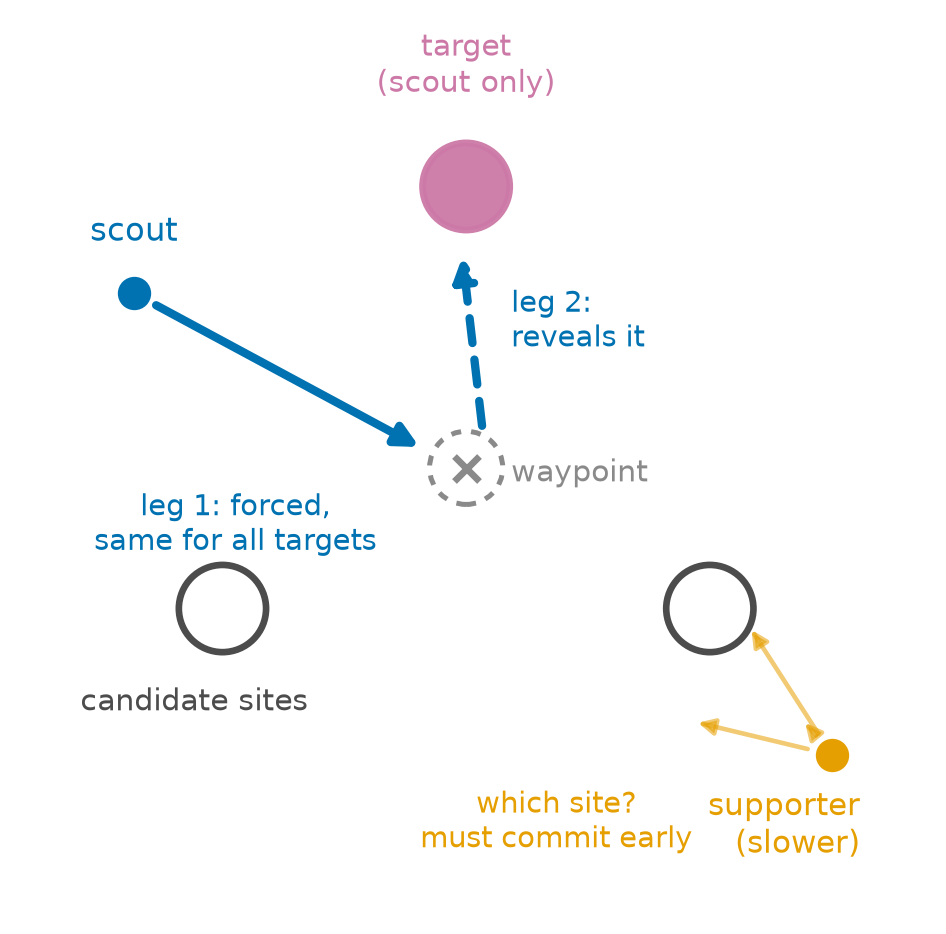
\includegraphics[width=0.80\columnwidth]{img/schematic.png}
\caption{Environment A, and why it can test legibility. The scout's forced first leg through the pickup waypoint is target-independent, so the target is revealed only on the second leg---after the slower supporter must already have committed.}
\label{fig:schematic}
\end{figure}

\textbf{Algorithm and conditions.} All agents train with multi-agent SAC: parameter-shared Gaussian actors, a centralized twin critic \cite{lowe2017multi} on the scalar team reward with $\lambda\Rcomm$ added, automatic entropy tuning. Conditions differ only in reward and observation content: baseline ($\lambda{=}0$), oracle, the four hand-crafted listeners, the learned family (literal, $+$RSA, bounded), \emph{ear} conditions appending a listener's posterior to the supporter's observation at execution (still decentralized-executable), and two external baselines---\emph{information regularization} after Strouse et al.~\cite{strouse2018learning} (reward $\log q_1(m|s,a) - \log q_0(m|s)$, two decoders, a variational $I(A;M|S)$) and a \emph{partner-belief} reward after Tian et al.~\cite{tian2020implicit} (a decoder over the supporter's own observation). $\lambda=0.3$ and the VOI weight were selected in preliminary short-budget sweeps on the standard task, then frozen for every transfer (Appendix~\ref{app:hyper}).

\textbf{Metrics and statistical policy.} We evaluate on a fixed 64-episode set (identical layouts across conditions and evaluations; cross-condition tests are unpaired Welch over seeds), average the last three evaluations, and train 400 cycles ($1.28$M steps) throughout. \emph{Commitment accuracy} is the fraction of steps the supporter's nearest site is the true target; \emph{post-hoc decodability} uses a fresh listener trained from scratch on each converged policy's rollouts. Headline claims have Welch $t \geq 4$, surviving Bonferroni at $\alpha{=}.05$ across the ${\sim}30$ condition-versus-baseline tests of Table~\ref{tab:scout}---the family we correct over; effects at conventional $p{<}.05$ are labeled suggestive and uncorrected. Negative claims meet the same bar: where a point estimate falls below baseline without clearing it, we report a null rather than a harm. Pre-registration means operationally that the launch specification was committed before any run of the cohort started, with confirmation cohorts held-out seeds under a frozen recipe. Seed counts grew by extension (never selective stopping); no completed run was excluded, and extensions are disclosed where they changed an estimate.

\section{Results}
\label{sec:results}

The ranking below is counterintuitive: it traces to the saturation Proposition~\ref{prop:saturation} predicts, and resolves into a listener nobody has to design.

\subsection{Environment A: Which Listener Pays}
\label{ssec:results_scout}

Table~\ref{tab:scout} and Fig.~\ref{fig:listeners} summarize Environment A at the matched $400$-cycle budget. The oracle premium---the irreducible value of early intent information---is $0.112$ per step ($0.957$ vs.\ $0.845$; commitment $.880$ vs.\ $.851$).

\textbf{Motion-grounded hand-crafted listeners close most of the gap.} The strongest conditions are the simplest: through the speaker-side reward alone, progress closes $70\%$ (Welch $t=6.2$), filter $67\%$ ($t=6.5$), plain cosine $62\%$ ($t=5.0$), with the largest commitment gains ($.857$--$.861$) and more legible scouts (geometric-probe accuracy $.61$ vs.\ $.54$ under a decoder external to every condition). They credit only \emph{overtly} geometric signals---exactly what the supporter's policy network reads from raw observations; the channel is the behavior itself. The exception proves the calibration rule: the exclusivity listener, whose margin demand is geometrically unsatisfiable, is unstable across seeds (a $1$-in-$8$ collapse rate: seven seeds in $0.84$--$0.93$, one at $0.23$; an early $n{=}3$ estimate of $+16\%$ closure was eliminated by extension to $n{=}8$).

\textbf{A blind-partner control supports the mechanism.} Masking the supporter's view of the scout (8 seeds; blind oracle 4), the pragmatic gain inverts into a significant cost ($-1.67$ vs.\ $-1.56$; $t=2.8$, $p\approx.02$, uncorrected)---the scout still pays the signaling detour for messages nobody receives---while the blind \emph{oracle} retains full performance ($0.963$). The effect is communication, not shaping.

\textbf{The supporter commits earlier, not merely correctly.} Terminal commitment is at ceiling everywhere, so the mechanism is timing. Pre-pickup ($t\le15$, full VOI weight) the oracle raises commitment accuracy by $.060$ ($t{=}22.8$); the inverse-planning listener recovers $41\%$ of that ($t{=}8.2$), progress $30\%$ ($t{=}4.7$), the inert learned listener none ($t{=}1.0$). The ordering is right but the mediation partial---filter closes $67\%$ of the reward premium on $11\%$ of this gap---so earlier commitment is one route to the gain, not all of it.

\textbf{A too-competent listener exerts no pressure.} Trained to convergence, the full-context $\Ltheta$ decodes the scout at $97\%$ \emph{whatever the scout does}: its reward saturates near the $\log 3$ ceiling and the speaker-side learned condition does not improve on baseline (the $-15\%$ point estimate is not significant, $t{=}{-}1.0$). Deployed as the supporter's \emph{ear} the same listener recovers $30\%$ ($t=2.15$, suggestive)---with a saturated listener the value is in the decoding, not the speaking---while adding an ear to a hand-crafted reward adds nothing over the reward alone.

\textbf{External baselines, head-to-head.} We run the two closest prior designs under the frozen recipe ($\lambda{=}0.3$, VOI, 8 seeds, 400 cycles). Tian et al.'s partner-belief reward~\cite{tian2020implicit}---a decoder over the supporter's own observation---lands at baseline parity ($6\%$ closure, n.s.) with a small commitment gain: fixing the audience to the actual partner's information state is exactly the saturating choice our analysis warns against. Strouse et al.'s information regularization~\cite{strouse2018learning}---$\log q_1(m|s,a) - \log q_0(m|s)$---closes $34\%$ ($t=2.6$, suggestive), indistinguishable from our bounded$+$RSA recipe, for a principled reason: subtracting the state decoder removes the contextual shortcut \emph{by construction}, implementing the viewpoint bound by subtraction where RSA implements it by contrast. Both designs received weight sweeps, and information regularization \emph{peaks} at $\lambda{=}0.3$ (falling to $3\%$ and $13\%$ at $\lambda{=}0.6$ and $1.0$, both n.s.) exactly where the recursion reward peaks at $\lambda{=}0.6$: the two context-debiasing routes have opposite weight tolerance. Under a common harness both designs thus sit in the same band at their optima and trail the vocabulary-restricted hand-crafted listeners by a factor of two---the second clause made quantitative.

\begin{figure}[t]
\centering
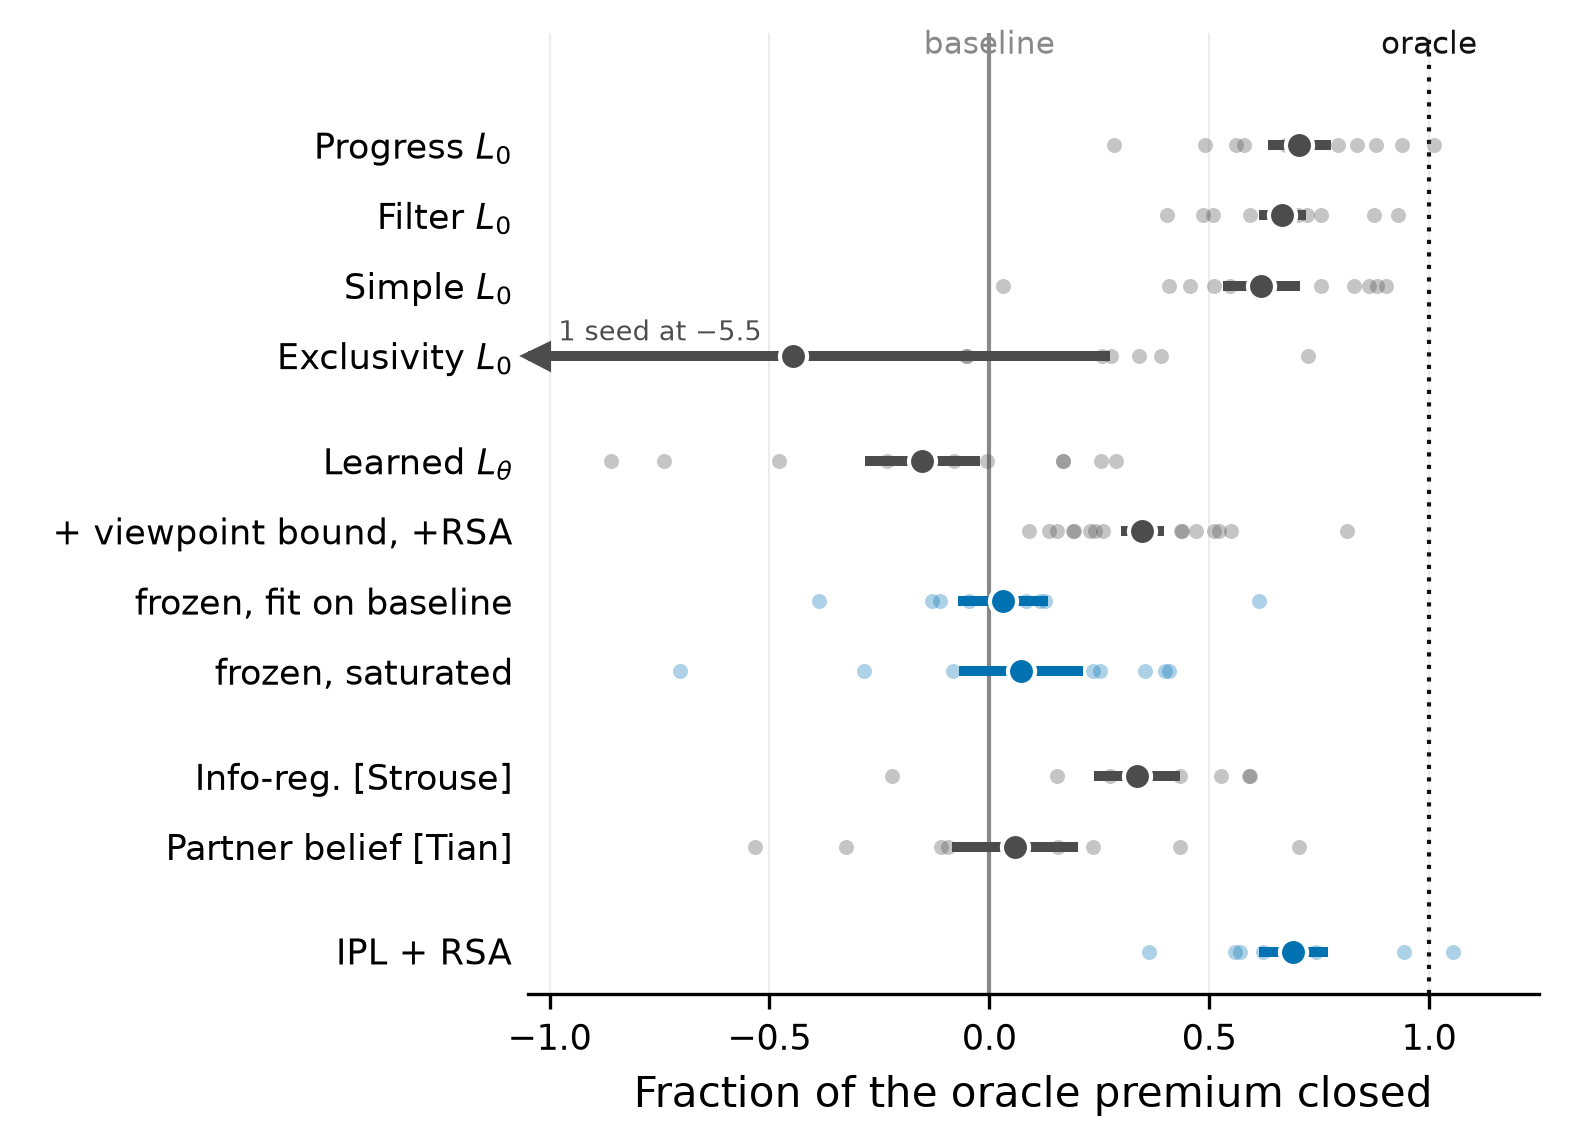
\includegraphics[width=\columnwidth]{img/listeners.png}
\caption{Which listener pays, in Environment A. Dots are seeds, bar $\pm1$ s.e.m., marker the mean; blue marks the rows the argument turns on. Exclusivity is bimodal rather than merely uncertain: seven seeds spread over closure $-.04$--$.76$, one far off-scale. Exact values in Table~\ref{tab:scout}; the two frozen ablations are in Sec.~\ref{ssec:results_scout}.}
\label{fig:listeners}
\end{figure}

\begin{table}[t]
\centering
\caption{Environment A at the matched $400$-cycle budget (mean $\pm$ s.e.m.; $3\times$-budget anchors: Sec.~\ref{ssec:results_dynamics}). Closure is the fraction of the oracle premium closed; Commit is the supporter's commitment accuracy. Closures shown only where $|t|\ge2$; otherwise n.s., in both directions. $n{=}10$ seeds unless marked $^\dagger${\,}($n{=}8$) or $^\ddagger${\,}($n{=}6$).}
\label{tab:scout}
\footnotesize
\setlength{\tabcolsep}{4pt}
\begin{tabular}{@{}>{\raggedright\arraybackslash}p{0.40\columnwidth}ccc@{}}
\toprule
\textbf{Condition} & $\Rext$ & Closure & Commit \\
\midrule
Baseline & $0.845\pm.010$ & --- & $.851$ \\
Oracle & $0.957\pm.008$ & $100\%$ & $.880$ \\
\midrule
Simple $L_0$ & $0.915\pm.010$ & $62\%$ & $.857$ \\
Exclusivity $L_0^\dagger$ & $0.795\pm.081$ & n.s. & $.850$ \\
Progress $L_0$ & $\mathbf{0.924\pm.008}$ & $\mathbf{70\%}$ & $\mathbf{.861}$ \\
Filter $L_0$ & $0.920\pm.006$ & $67\%$ & $.858$ \\
\midrule
Learned $\Ltheta$ & $0.828\pm.015$ & n.s. & $.853$ \\
Learned $+$ RSA$^\dagger$ & $0.863\pm.008$ & n.s. & $.856$ \\
Bounded $+$ RSA ($\lambda{=}.6$)$^\dagger$ & $0.875\pm.005$ & $27\%$ & $.861$ \\
\midrule
IPL, literal$^\dagger$ & $0.907\pm.014$ & $55\%$ & $.864$ \\
IPL $+$ RSA ($\lambda{=}.3$)$^\dagger$ & $0.919\pm.006$ & $66\%$ & $.862$ \\
IPL $+$ RSA ($\lambda{=}.6$)$^\dagger$ & $\mathbf{0.923\pm.009}$ & $\mathbf{70\%}$ & $\mathbf{.863}$ \\
\midrule
Info-reg.\ \cite{strouse2018learning}$^\dagger$ & $0.883\pm.011$ & $34\%$ & $.856$ \\
Partner belief \cite{tian2020implicit}$^\dagger$ & $0.852\pm.016$ & n.s. & $.856$ \\
\midrule
Ear, $\lambda{=}0^\ddagger$ & $0.874\pm.016$ & n.s. & $.854$ \\
Ear $+$ $\Rcomm$ & $0.878\pm.012$ & $30\%$ & $.858$ \\
Filter $+$ ear & $0.920\pm.012$ & $66\%$ & $.854$ \\
\bottomrule
\end{tabular}
\end{table}

\subsubsection{Bounding the Learned Listener}
\label{ssec:results_bounded}

If the learned listener fails because it is too strong, the obvious remedy is to weaken it toward the intended reader. A \emph{viewpoint-bounded} listener sees only site bearings and the action---what the audience uses to interpret the utterance---removing the contextual shortcut; a \emph{window-bounded} variant additionally trains only on pre-commitment steps, so decode accuracy cannot be earned from the post-commitment leg (Fig.~\ref{fig:listeners}).

The first is a negative control that sharpens the principle. Both bounded listeners \emph{re-saturate}---later (decode accuracy $0.54$ at quarter-training for window-bounded vs.\ $0.88$ full-context) and by the second route of Proposition~\ref{prop:saturation}, co-adapting to whatever the policy emits. Their literal rewards end at baseline parity, curing the harm but recovering nothing. Layering RSA recursion on top lands at $0.868$ ($21\%$ closure) in two replications, ahead of its literal counterpart at all but one evaluation.

The second is the cleanest causal contrast. Raising the weight ($\lambda{=}0.6$, the middle of three swept) lifted the recursed variant to $0.893\pm.009$ ($43\%$) on the selection runs; eight held-out confirmation seeds showed the expected regression to the mean (Sec.~\ref{ssec:results_dynamics}). Since the selection cohort chose $\lambda$, the confirmation cohort is primary: $27\%$ closure ($t=2.7$); pooling gives $0.884\pm.006$ ($35\%$, $t=3.4$) but re-imports the selection bias (secondary). The control is decisive: the \emph{literal} listener at the same weight does not rise above baseline ($0.820\pm.016$, n.s.), so amplifying a saturated reward buys nothing even as the recursed variant gains. Recursion vs.\ none at matched weight is worth $0.055$ ($t{=}3.3$) against the primary estimate, replicated in direction across four cohorts. The deployed-ear variant is redundant by construction and lands at baseline parity ($0.841\pm.023$; an earlier catastrophic estimate was an evaluation bug disclosed in the appendix).

Why the residual gap to the hand-crafted family ($27\%$ vs.\ $70\%$)? A co-adapting listener stays satisfied by \emph{any} decodable regularity, including idiosyncratic codes the co-training supporter tracks imperfectly.

\textbf{The inverse-planning listener closes the gap.} That failure motivates the construction deferred in Sec.~\ref{ssec:listeners}: freeze a non-communicative baseline and Bayes-invert it. The IPL resolves the residual outright with no hand-crafted geometry---its literal form closes $55\%$ ($t=3.6$), and one RSA step reaches $66\%$ at $\lambda{=}0.3$ ($t=6.3$) and $\mathbf{70\%}$ at $\lambda{=}0.6$ ($t=5.8$), in the progress listener's band, with commitment $.862$--$.864$. Both recursed points clear the $t\ge4$ bar, the first learned-family results here to do so. Two weights were run and both are reported; unlike the bounded listener the IPL has no held-out confirmation cohort, so the $70\%$ endpoint carries a residual selection caveat at two-point scale. A post-hoc depth sweep ($N_r{\in}{\{}2,3,5{\}}$, 8 seeds each, matched budget) is flat---$79\%$, $81\%$, $70\%$ closure, pairwise $|t|{\le}1.4$---and pooling all 32 recursed seeds against the literal leaves the increment unresolved ($t{=}1.5$): the grounding carries the effect, and depth is not a tuned knob. The inversion is well-specified here, not merely convenient: a converged SAC policy is itself Boltzmann-rational ($\pi(a|s)\propto\exp(Q(s,a)/\alpha)$), so the soft rationality the listener assumes is the speaker's \emph{true} policy class---and entropy regularization prices away costless determinism, so the structure that survives in behavior is structure the critic pays for. What the bounded listeners lacked was never hand-crafted geometry but a \emph{non-co-adapting, competence-grounded} literal listener. The recipe for any goal-conditioned task: train without communication, freeze, Bayes-invert at soft rationality, add the recursion.

\textbf{Freezing alone is not the mechanism.} The IPL is both frozen and anchored in a task-competent reference; two ablations separate these. Fitting the same bounded listener by maximum likelihood on rollouts of the \emph{same} frozen baseline and then freezing it closes $3.2\%$ ($0.849\pm.012$, $t{=}0.2$); freezing the converged full-context listener as a static reward closes $7.3\%$ ($0.853\pm.016$, $t{=}0.4$). Neither is distinguishable from baseline, and both are beaten by the still \emph{co-adapting} bounded listener with recursion ($34.8\%$): what separates the IPL is what its listener credits, not that it stopped moving. The first ablation shows why---a decoder fit to a non-communicative policy has little to learn (held-out accuracy $.44$ against $.33$ chance), whereas the IPL never needs signal present in the data, since it queries the reference policy counterfactually under each candidate meaning. Clause (b) is thus a tested condition for the IPL's success, not an interpretation of it.

\textbf{One recipe, three task variants; robustness.} The recipe (progress, $\lambda{=}0.3$, VOI, frozen) transfers untuned to two structurally distinct variants of the family ($n{=}8$ seeds each): five meanings closes $82\%$ ($t=3.98$, $p=.0014$, surviving Bonferroni), minefield $61\%$ ($t=5.2$, $p<.001$), majority-gap closure in both. It is a plateau, not a tuned point: $0.894$--$0.925$ across the $\lambda \in \{0.1,0.3\}\times$VOI grid (low end at $\lambda{=}0.1$, uniform weighting; 3 seeds/cell), with a cliff at $\lambda{=}0.6$ under VOI weighting ($0.450\pm.203$; $0.823$ uniform)---the \emph{optimum} $\lambda$ for the bounded learned-pragmatic reward: the safe weight range scales inversely with reward magnitude.

\subsubsection{The Signal Is Grounded, Not Conventional}
\label{ssec:readers}

A converged baseline could coordinate through an emergent code of its own---readable by its co-trained partner yet opaque to everyone else---so whether legibility rewards create meaning or amplify it turns on what the pre-key signal is grounded in. We read each converged policy's forced first leg with four readers ordered by grounding (Table~\ref{tab:readers}): the fixed geometric probe (a human prior about motion), the inverse-planning listener (a frozen non-communicative policy from a disjoint seed), and a decoder of the paper's bounded family fitted either to held-out rollouts of the same seed or to the seven sibling seeds at matched sample budget. Every reader sees only scout kinematics and the action, with the meaning slot zeroed as in the IPL's counterfactuals.

Three facts fall out. First, \emph{every} policy leaks: the baseline's forced leg is already $74\%$ decodable by a fitted reader---most of the meaning is in the motion of any competent agent before the environment reveals anything, which is exactly the saturating common ground a maximum-likelihood listener converges to (Sec.~\ref{ssec:results_bounded}). Second, the leak is shared, not private: a decoder fitted to sibling seeds reads each policy as well as its own decoder does ($|t|{\le}1.5$ everywhere), and the frozen-policy reader recovers $90$--$97\%$ of whatever the fitted one finds (for the oracle, more than all of it). No equilibrium-specific convention appears in any condition---consistent with max-ent training, which prices away costless determinism: a private code that earned nothing through the partner would not survive the entropy bonus, and one that did would be seed-specific, which is what we do not observe. Third, incentive moves the \emph{amount} of grounded signal, not its kind: total pre-key decodability orders IPL$+$RSA ($.86$) $>$ progress ($.83$) $>$ baseline ($.74$) $>$ oracle ($.55$), the residue beyond the human prior orders the same way ($.43/.42/.33/.13$; progress vs.\ baseline $t{=}6.7$), and the oracle---whose partner already knows---is the least readable agent in the study. The two winning anchors amplify in their \emph{own} vocabularies: the progress-shaped scout gains most under the geometric prior ($+.07$) while the IPL-shaped scout is flat there ($+.01$, n.s.) yet gains $+.09$ under the competence reader ($t{=}9.3$)---the audience question is symmetric, and a probe is an audience too. The pragmatic reward amplifies a transferable, competence-grounded signal latent in task behavior; it does not invent a code. (Fitted readers are capacity-bounded, so totals are lower bounds; the ordering holds in-sample as well, $.92/.86/.72$.)

Two boundary notes. The forced-leg signal is integrated deviation, not instantaneous direction: the geometric probe reads ${\approx}.41$ there in every condition and acquires its progress-vs-baseline gap only post-key ($.69$ vs.\ $.60$), while the IPL orders the conditions pre-key already---which is why the history-integrating listeners succeed where an instantaneous prior cannot. And reading the \emph{pair} instead of the scout inflates every number ($.85$--$.91$, oracle highest, through the supporter's drift toward the answer)---precisely the channel the blind control severs. Timing is matched throughout (pickup at $9.7$--$10.1$ steps, the rewarded scouts marginally \emph{later}): earlier supporter commitment is earned by reading motion, not bought by an earlier reveal.

\begin{table}[t]
\centering
\caption{Reading the forced first leg, readers ordered by grounding (pre-key accuracy; chance $1/3$; $n{=}8$ seeds, s.e.\ $\le.013$). Fitted readers are evaluated on held-out episodes; ``other seeds'' is fitted to the seven siblings at matched sample budget. Own-seed and other-seed readers agree in every condition ($|t|{\le}1.5$): no equilibrium-specific code.}
\label{tab:readers}
\small
\setlength{\tabcolsep}{5pt}
\begin{tabular}{@{}lcccc@{}}
\toprule
\textbf{Reader (grounding)} & Baseline & Oracle & Progress & IPL$+$RSA \\
\midrule
Geometric (human prior) & $.419$ & $.418$ & $.411$ & $.433$ \\
IPL (frozen policy) & $.720$ & $.626$ & $.749$ & $.812$ \\
Fitted, own seed & $.742$ & $.547$ & $.829$ & $.857$ \\
Fitted, other seeds & $.720$ & $.537$ & $.820$ & $.848$ \\
\bottomrule
\end{tabular}
\end{table}

\subsection{When Does Pragmatism Pay? A Boundary Map}
\label{ssec:boundary}

We vary the two quantities that should govern the effect---what early intent is worth (partner speed $0.45$--$0.90$ sets the oracle premium) and what signaling costs (scout shaping weight $2\times$, $4\times$)---at 5 seeds per setting, everything else frozen, and plot all settings on premium-vs-gain axes (Fig.~\ref{fig:boundary}).

\textbf{An empirical regularity, stated with its scope.} Wherever the premium is resolvable (point estimate $>3\times$ its s.e., fixed before analysis), the recipe captures a roughly constant fraction: an origin-constrained fit over all seven resolvable settings gives $\text{gain} \approx 0.51 \times \text{premium}$ (bootstrap $95\%$ CI $[0.42, 0.59]$). It is an observation, not a law. The two failure-mode settings below have the \emph{largest} premiums and dominate the fit; excluding them gives $0.68\times$, but that split is post hoc ($0.51$ primary, $0.68$ exploratory). Gain and premium also share each setting's baseline estimate, so their errors correlate. Seven points from one environment family and one algorithm establish a regularity of that family, falsifiable by any resolvable-premium, healthy-channel environment capturing outside the fitted range.

\textbf{Failure modes.} Where no premium is resolvable, no gain appears (preference spread $t{=}0.2$ at the converged budget; $4\times$ cost $t{=}1.4$). Where it is real but the partner too slow ($0.45$) or signaling too expensive ($2\times$), capture drops to $0.37\times$: the premium is partly unreachable at any signaling latency, or the scout rationally emits less. Where the channel is severed (blind), the reward does not merely stop helping but \emph{hurts}, the speaker paying for signals nobody receives.

\textbf{The boundary is two-sided: something to say, and not already said.} A highway on-ramp negotiation, built as a candidate third environment, closed the boundary from the far side: the merger's \emph{task-optimal} approach---aligning with its intended gap---is inherently informative, and baseline RL bootstrapped meaning-differentiated accommodation unaided, listeners braking selectively for the correct gap under no communicative reward, leaving the oracle premium unresolvable ($0.021\approx1.3\times$ s.e.) even though severing the channel cost 26 points of success. \emph{Signal pre-existence} mirrors Environment B's failure mode: legibility rewards buy value only when the agent has something to say (else they purchase certified miscalibration, Sec.~\ref{ssec:results_spread}) \emph{and} the task does not already say it (else optimization substitutes for communication). We report this as a negative result because it is one; so is a three-lane fork in which cooperators must open a corridor for a merging vehicle, built to repair the on-ramp's weaknesses and also failing the gate at $800$ cycles (baseline $0.361\pm.060$ vs.\ oracle $0.368\pm.079$, $n{=}4$), the cooperators again converging on accommodation unaided. Two independent attempts at a second premium-positive environment thus failed---the strongest evidence we can offer that the gate is not a formality, and a real limit on the external validity of everything following from the one family that passed. The $0.51\times$ regularity quantifies the region between, its pre-registered scope the partner-speed/cost family: the meaning-space regimes of Sec.~\ref{ssec:continuous} fall below the fitted band (capture $0.18$--$0.26$), read as the axis along which certification weakens, not a violation of the within-family fit.

\subsubsection{The Pre-Convergence Hazard}
\label{ssec:results_dynamics}

This benchmark produced three successive spurious conclusions before the converged one. At increasing budgets (Fig.~\ref{fig:budget}) the progress listener's effect reads as strongly negative through $0.5$M steps ($\approx{-}60\%$ closure at our early budget) and $+70\%$ only past ${\sim}1$M; at 150 of the ${\sim}400$ needed cycles hand-crafted listeners appeared destructive while an ear condition appeared to close $30\%$ of a then-larger gap---evaporating when seeds were doubled. Communicative-MARL comparisons are unusually exposed because the quantity of interest is a co-adaptation between policies and listeners, converging more slowly than either alone; we recommend reporting training-stage sensitivity as in Fig.~\ref{fig:budget}.

Applying the discipline to ourselves cost the headline its gloss. The 400-cycle diagnostics that motivated an extension (oracle plateaued; baseline still climbing at $t{=}3.9$) resolve, at $3\times$ budget (Fig.~\ref{fig:convergence}), into a second-order form of the hazard our own convergence check missed: the \emph{ordering} stabilizes by 400 cycles, the \emph{magnitude} does not. The premium peaks near $1.45$ around cycle 80---while the baseline is still near its floor, so most of what privileged information buys early is learning speed---then settles at $0.073$ ($t{=}7.7$ over cycles 800--1200, $n{=}8$): communication has genuine asymptotic task value, but the 400-cycle premium of $0.130$ is $1.8\times$ its converged size. The progress listener's capture falls with it, $72\%$ $[59,87]$ to $36\%$ $[10,59]$ ($t{=}9.9$ to $2.4$), and the pattern is family-wide (Table~\ref{tab:budget}): every grounded anchor keeps a suggestive-tier converged gain (filter $+.020$, IPL $+.028$; $t{=}2.3$--$2.7$) while the co-adapting learned listener keeps none ($+.004$, $t{=}0.4$, fresh seeds replicating its 400-cycle null)---the dissociation survives the asymptote, though its head-to-head contrasts there sit at the edge of eight-seed resolution ($t{\approx}1.8$--$2.3$). At long budgets the absolute gain ($0.093$ to $0.026$ reward/step) is the primary statistic: its seed spread is unchanged ($0.021$ vs.\ $0.023$) and the capture interval widens exactly as the shrinking denominator predicts ($\times2.00$ predicted, $\times2.00$ observed), so at the asymptote the ratio is the noisier statistic, not the more honest one.

\begin{table}[t]
\centering
\caption{The dissociation survives the asymptote. Gains over baseline (reward/step, Welch $t$) in the 400-cycle evaluation window (premium $0.130$) and at convergence (cycles 800--1200, premium $0.073$), and the converged readability gap under the fixed probe. $n{=}8$ everywhere; learned and filter are fresh seeds at both budgets.}
\label{tab:budget}
\small
\setlength{\tabcolsep}{3.5pt}
\begin{tabular}{@{}lccccc@{}}
\toprule
 & \multicolumn{2}{c}{At 400 cycles} & \multicolumn{2}{c}{At convergence} & Probe gap \\
\cmidrule(lr){2-3}\cmidrule(lr){4-5}
\textbf{Condition} & gain ($t$) & capt. & gain ($t$) & capt. & at conv.\ ($t$) \\
\midrule
Oracle & $+.130$ (12.0) & $100\%$ & $+.073$ (7.7) & $100\%$ & $-.082$ ($-2.8$) \\
Progress $L_0$ & $+.093$ (9.9) & $72\%$ & $+.026$ (2.4) & $36\%$ & $+.071$ (3.2) \\
Filter $L_0$ & $+.081$ (8.0) & $62\%$ & $+.020$ (2.3) & $28\%$ & $+.077$ (4.0) \\
IPL $+$ RSA & $+.081$ (7.1) & $62\%$ & $+.028$ (2.7) & $38\%$ & $-.025$ (n.s.) \\
Learned $\Ltheta$ & $-.004$ ($-0.3$) & n.s. & $+.004$ (0.4) & n.s. & $-.032$ ($-1.7$) \\
\bottomrule
\end{tabular}
\end{table}

What survives the extension is the paper's actual object. The fixed-probe readability gap \emph{widens} as the reward gap decays: $+.047$ ($t{=}3.4$) at the 400-cycle budget, $+.071$ ($t{=}3.2$) at convergence, with the baseline flat at $.55$ throughout and the oracle---the one agent with no incentive to signal---declining to $.47$, below baseline (Fig.~\ref{fig:legibility}; probe cross-entropy agrees at 400 cycles, $t{=}{-}5.7$, and is null at 1200, $t{=}1.3$). The gap is indexed to the paying listener's vocabulary: the IPL-shaped scout is flat to this human-prior probe ($-.02$, n.s.) yet carries the most total readable signal in the study ($.86$ to fitted readers; $+.09$ to the competence reader, $t{=}9.3$; Table~\ref{tab:readers}). At convergence the ordering sharpens: filter's readability gap is the largest and clears the headline bar ($+.077$, $t{=}4.0$) on the smallest surviving task gain, while the learned listener's is, if anything, negative ($-.032$, $t{=}{-}1.7$)---a listener trained to read everything teaches nothing. Legibility, not the task-reward margin, is the durable product of the reward; the margin it buys is concentrated where goal information is scarcest, early in joint training.


\begin{figure*}[t]
\centering
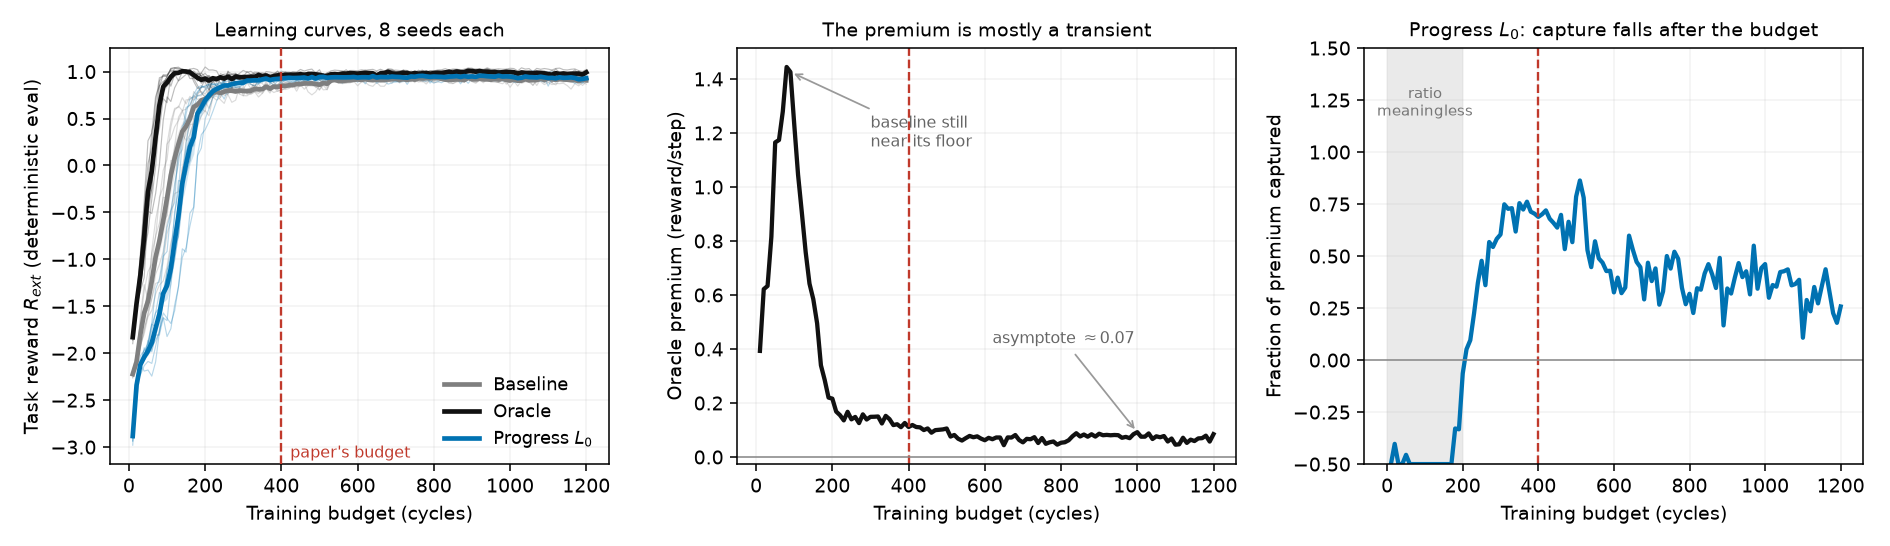
\includegraphics[width=0.98\textwidth]{img/convergence.png}
\caption{Three times past the evaluation budget (8 seeds per condition; dashed red: the 400-cycle budget). \textbf{Left:} per-seed learning curves; all conditions converge into one band. \textbf{Middle:} the oracle premium spikes near $1.45$ while the baseline is still near its floor---early privileged information mostly buys learning speed---then settles at ${\approx}0.073$. \textbf{Right:} the fraction of the premium the progress listener captures peaks near the evaluation budget and settles near one third; the ratio is greyed out where its denominator is unresolved.}
\label{fig:convergence}
\end{figure*}

\begin{figure*}[t]
\centering
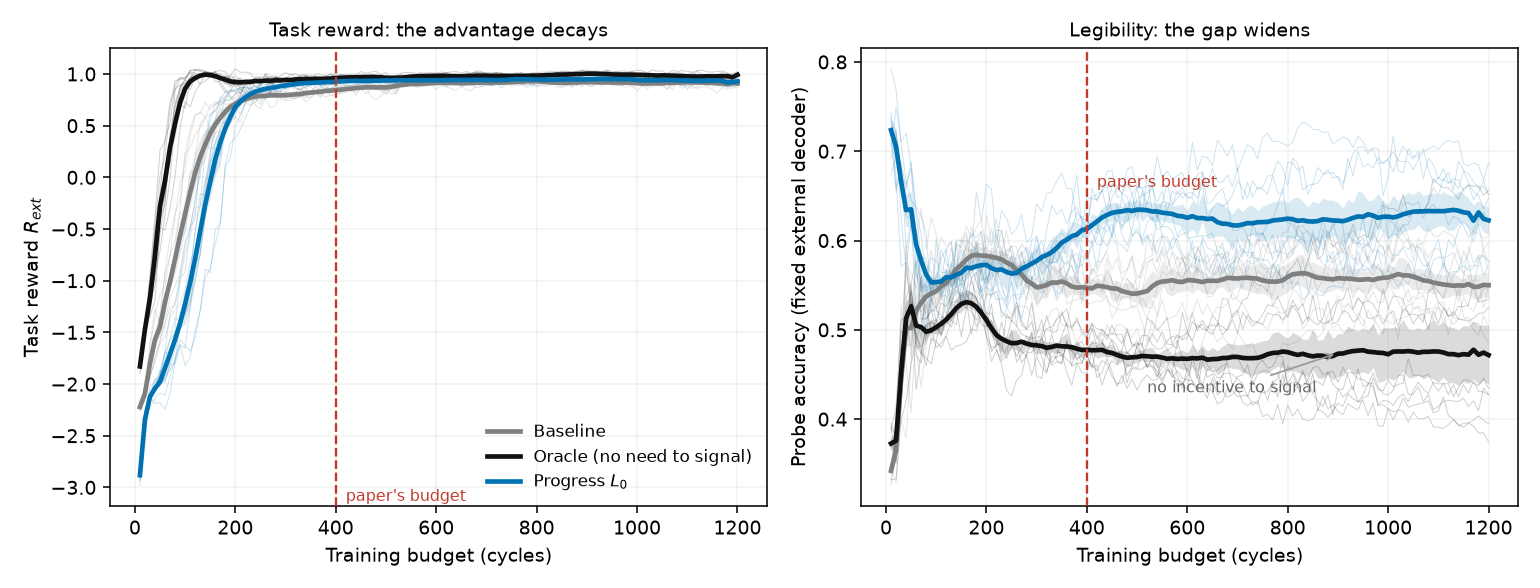
\includegraphics[width=0.92\textwidth]{img/legibility.png}
\caption{What decays and what survives (per-seed traces behind the means). \textbf{Left:} the task-reward advantage is transient---the baseline converges into the same band. \textbf{Right:} readability by a fixed external decoder diverges instead: the pragmatic scout climbs and holds, the baseline stays flat, and the oracle, whose partner already knows the target, sheds even incidental readability.}
\label{fig:legibility}
\end{figure*}

\subsection{Environment B: The Cost of Signaling with Nothing to Say}
\label{ssec:results_spread}

Environment B (converged 400-cycle budget, 5 seeds; full numbers in Appendix~\ref{app:envb}) confirms the near-zero premium by oracle ($1.93$ vs.\ $1.86$, $+0.07\pm.08$, n.s.; an earlier 150-cycle evaluation put the oracle \emph{below} baseline---the pre-convergence hazard of Sec.~\ref{ssec:results_dynamics}, which also inflated the miscalibration tax below from $9\%$ to $46\%$). Calibrated learned listeners are a free add-on: task reward at baseline ($1.93\pm.06$ literal, $1.87\pm.02$ recursed), communicative reward at genuinely \emph{positive} information gain ($+0.21$/$+0.22$), the recursion again extracting more decodable signal than literal decoding (listener accuracy $.681$ vs.\ $.655$). Miscalibration is a tax with a free diagnostic: the exclusivity listener's own reward is stuck \emph{below} the uninformative level ($-1.83$; its margin demand is geometrically unsatisfiable) and it costs $9\%$ of task reward ($1.69$, $t=2.3$, suggestive). A post-hoc coda shows the tax is a vocabulary mismatch, not an absence of signal: that condition's behavior is the \emph{most} decodable of all to a fresh probe ($.700\pm.008$ vs.\ $.665\pm.007$, $t=3.2$, uncorrected), yet its own listener never credits it---so a reward persistently below its uninformative level certifies miscalibration at zero cost.

\subsection{The Meaning-Space Axis: Discrete, Continuous, Self-Assigned}
\label{ssec:continuous}

Varying the meaning space itself---discrete labels, a continuum, then a latent the agent assigns itself---the paper's ordering replicates in all three: the literal listener is inert, one recursion step lifts it, and the advantage never reverses sign (Fig.~\ref{fig:meaning_axis}). Its \emph{magnitude} is decisive only in the discrete regime ($t{\ge}5.8$); continuous and self-assigned closures are suggestive ($t{=}2.2$--$2.3$) and we label them so throughout. Appendix~\ref{app:meaning} gives the estimator, the per-cohort numbers, and the probe protocol; Appendix~\ref{app:figs} collects the supporting figures.

\textbf{Continuous meanings.} What breaks on a continuum is not the decoder but the recursion, whose listener normalization integrates over $\mathcal{M}$. We replace it with \emph{contrast particles}---the true meaning scored against $K{=}15$ alternatives drawn from other episodes in the batch---so both normalizations become finite softmaxes and the recursion becomes alternating row/column scaling: steps of the Sinkhorn scaling that Wang et al.\ identify as the mathematical form of cooperative-communication recursions, RSA included \cite{wang2020cooperative}. At zero depth the objective is \emph{exactly} InfoNCE \cite{oord2018representation} at the true meaning, so Propositions~\ref{prop:mi} and \ref{prop:saturation} carry over with a $\log(K{+}1)$ ceiling in place of $\log|\mathcal{M}|$; sampled-alternative RSA is familiar from pragmatic captioning \cite{cohngordon2018pragmatically}. Our contribution is the estimator, not the identification. On a continuous-bearing scout-support ($\mathcal{M}=S^1$) the premium re-certifies ($0.843\pm.007$ vs.\ $0.945\pm.008$, $n{=}8$; blind commitment at chance): the literal contrastive listener is inert ($4.9\%$, $t{=}0.5$) even as its decoder concentrates (top-1 $.74$ against a $.06$ chance level---the saturation signature again), while one Sinkhorn iteration closes $17.7\%$ (pooled $n{=}16$, $t{=}2.2$). Density is itself a finding: the progress listener, ported for free by scoring particles, drops from $70\%$ to $15.8\%$ ($t{=}1.6$). When meanings are dense, nearby ones have near-identical action consequences and \emph{every} listener family captures less---an extension of the boundary map, not a property of any one listener.

\textbf{Self-assigned meanings: legible latents.} The last step drops the assumption that the meaning is given. The scout's private observation---enriched with two decoy bearings and two noise channels, only the true bearing decision-relevant---now reaches its policy only through a variational encoder, so the latent $z$ is the only route from private information to behavior and what it carries is decided by task pressure and compression rather than by us. The wiring is InfoBot's \cite{goyal2019infobot} sign-flipped, and the reward mechanism has a free-latent ancestor in Any-Play's teammate-side skill discriminator \cite{lucas2022anyplay}; all conditions share the architecture and $\beta$, so the anchors price communication, not capacity. Aiming the particle recursion at the speaker's own per-episode posterior mean makes the representation that drives its decisions readable from how it acts, and the premium survives the inversion---an oracle advantage for a latent the designer never specified ($1.001\pm.006$ vs.\ $1.089\pm.013$, $n{=}8$, $6\times$ s.e.; blind commitment near chance). The ordering replicates a fourth time with no hand-specified meaning anywhere in the loop: the literal reward is inert ($8.5\%$, $t{=}0.8$) while one Sinkhorn iteration closes $25.7\%$ ($t{=}2.3$, suggestive). Post-hoc probes then separate what the latent carries from how much of it shows. The true bearing is linearly decodable from $z$ at $R^2{=}.999$ in \emph{every} condition, while $I(Z;\text{behavior})$ tracks the same ordering as the task results---$1.762\pm.004$ at baseline, $1.781$ under the literal reward, $1.814\pm.010$ under the recursion ($t{=}4.6$)---and the VIB rate, a variational \emph{upper} bound on $I(Z;\text{private})$, stays statistically indistinguishable across the three ($10.61$, $10.55$, $10.54$ nats). Compression and task pressure choose \emph{what} enters $z$; the pragmatic reward chooses \emph{how much of it shows} (Fig.~\ref{fig:transparency}). To our knowledge the certified premium for an information-bearing \emph{learned} latent, and this content-versus-exposure dissociation (cf.\ amnesic probing \cite{elazar2021amnesic}), appear here first; the nearest relative, VQ-VIB \cite{tucker2022trading}, learns such a latent but over an explicit channel with no behavior-legibility reward or certification, while prior exposure-direction rewards target \emph{given} private variables \cite{strouse2018learning,tian2020implicit,fuchs2021theory,liu2025active,faylor2025teammates} and prior latent-discriminability rewards target \emph{free} skill noise \cite{eysenbach2019diversity,lucas2022anyplay}.

\section{Discussion}
\label{sec:discussion}

The results converge on one design constraint, opposite to the intuition that a better model of the audience makes a better reward. The learned listener decodes the scout at $97\%$ regardless of behavior, and what remains of its reward's variation is no smaller than the IPL's ($0.18$ action-conditional, for both)---but it points nowhere durable: fitting to the speaker's own data makes the code chase the policy, where the counterfactual anchor gives improvement a fixed target (Proposition~\ref{prop:saturation} bounds the fitted family's gradient, loosely at the measured operating point; it does not price the difference in direction); bounding it to the audience's viewpoint and decision window is necessary but not sufficient, since a bounded co-adapting listener still saturates on whatever code the policy emits. Calibration is what causes this: fitting $\Ltheta$ to the agents' own data guarantees the common ground never demands what the policy cannot express, which is why it optimizes smoothly and costs nothing where there is nothing to say (Environment B), and why, where there \emph{is}, the closer it converges to the posterior the less that posterior varies with behavior. What separates the crude geometric listeners is what they can credit: overtly geometric motion a feed-forward teammate reading raw observations can also exploit. An omniscient audience needs no speech; an infinitely accommodating one accepts any private code. The principle is therefore not ``model your audience accurately''---the maximum-likelihood listener is provably the \emph{most} accurate model of what behavior reveals (Proposition~\ref{prop:mi}), the partner-belief reward uses the true audience itself, and both are inert. Nor is it ``freeze the listener'': fitted to a frozen reference's rollouts, a listener is as inert as one fitted to the speaker's own. Every construction that works---geometric and inverse-planning alike---instead assembles the posterior from \emph{meaning-conditioned counterfactuals}: what would be done were the target $m'$ rather than $m$, at the same state. Fitting estimates $p(m\mid s,a)$ from data where the meaning is already legible in the context; counterfactual anchoring lets it move only with what the action discriminates---the quantity the reader can exploit. Non-saturation (Proposition~\ref{prop:saturation}) and reader-visible vocabulary (Proposition~\ref{prop:vocab}) follow from the construction rather than constraining it; exclusivity, which satisfies both yet demands a margin no trajectory supplies, fails for a separate third reason. What survives learning is RSA's recursion, converting an inert decoder into a reward recovering a quarter of the premium: the converged posterior no longer varies with behavior, but the contrast against foregone alternatives still does.

\textbf{Limitations.} Intrinsic rewards densify learning signals, and the $3\times$-budget extension quantifies the split rather than eliminating it: roughly half the evaluation-budget premium is learning speed, and the durable dividend is legibility (Sec.~\ref{ssec:results_dynamics}), with commitment timing and external probes carrying the attribution. The principle is demonstrated for one audience class (feed-forward policies over raw observations), one environment family, and one algorithm; how listener competence should scale with reader competence is open. Meanings are hand-specified in the headline results; Section~\ref{ssec:continuous} relaxes discreteness and then hand-specification, but closures there fall to the suggestive band, and both the meaning-space geometries that support legibility rewards and a pre-registered second-environment replication of the self-assigned regime remain open. Validation is confined to AI--AI teams; the principle predicts rewards anchored in human-competence listeners should transfer best to human-agent teams. Inverting $\lambda$'s sign turns legibility into obfuscation, suggesting privacy applications \cite{strouse2018learning}.

\section{Conclusion}
\label{sec:conclusion}

We connected pragmatic inference and maximum-entropy RL, importing the RSA listener value as an intrinsic reward for legible behavior whose decisive design choice is the literal listener. Where communication has no task value, miscalibrated listeners charge for undecodable signaling and calibrated ones approach a no-op. Where it is certifiably valuable, crude motion-grounded listeners that credit only overt signals recover $61$--$82\%$ of the oracle premium, while a listener competent enough to decode anything demands nothing---a failure our saturation bound describes, if loosely, at the directly measured operating point. Bounding the co-adapting learned listener cures its harm but not its inertness; the \emph{inverse-planning listener}---a Boltzmann observer self-instantiated from a frozen non-communicative baseline, sharpened by one RSA step---closes $55$--$70\%$ with no task-specific geometry while remaining human-readable. Counterfactual anchoring is RSA's oldest lesson restated for reward design: speech is optimized against a literal listener whose readings of the alternatives are constructed rather than learned from the speaker's own habits. The recipe is general---train the task without communication, freeze the policy, Bayes-invert it, let pragmatics do the rest---and reaches past given meanings, a bottleneck making an agent's own decision variable legible. Agents whose competence includes being understood must be trained against audiences that need the help.

\bibliographystyle{ACM-Reference-Format}
\begin{thebibliography}{10}

\bibitem{dragan2013legibility}
Anca~D. Dragan, Kenton~C.T. Lee, and Siddhartha~S. Srinivasa.
\newblock Legibility and predictability of robot motion.
\newblock In {\em HRI}, 2013.

\bibitem{goodman2016pragmatic}
Noah~D. Goodman and Michael~C. Frank.
\newblock Pragmatic language interpretation as probabilistic inference.
\newblock {\em Trends in Cognitive Sciences}, 20(11):818--829, 2016.

\bibitem{estienne2025collaborative}
Lautaro Estienne, Gabriel Ben~Zenou, Nona Naderi, Jackie~Chi~Kit Cheung, and Pablo Piantanida.
\newblock Collaborative rational speech act: Pragmatic reasoning for multi-turn dialog.
\newblock In {\em EMNLP}, 2025.

\bibitem{strouse2018learning}
DJ~Strouse, Max Kleiman-Weiner, Josh Tenenbaum, Matt Botvinick, and David~J. Schwab.
\newblock Learning to share and hide intentions using information regularization.
\newblock In {\em NeurIPS}, 2018.

\bibitem{goyal2019infobot}
Anirudh Goyal, Riashat Islam, DJ~Strouse, Zafarali Ahmed, Matthew Botvinick, Hugo Larochelle, Yoshua Bengio, and Sergey Levine.
\newblock InfoBot: Transfer and exploration via the information bottleneck.
\newblock In {\em ICLR}, 2019.

\bibitem{lucas2022anyplay}
Keane Lucas and Ross~E. Allen.
\newblock Any-Play: An intrinsic augmentation for zero-shot coordination.
\newblock In {\em AAMAS}, 2022.

\bibitem{tucker2022trading}
Mycal Tucker, Roger Levy, Julie Shah, and Noga Zaslavsky.
\newblock Trading off utility, informativeness, and complexity in emergent communication.
\newblock In {\em NeurIPS}, 2022.

\bibitem{elazar2021amnesic}
Yanai Elazar, Shauli Ravfogel, Alon Jacovi, and Yoav Goldberg.
\newblock Amnesic probing: Behavioral explanation with amnesic counterfactuals.
\newblock {\em TACL}, 9:160--175, 2021.

\bibitem{faylor2025teammates}
Miguel Faria, Francisco~S. Melo, and Ana Paiva.
\newblock ``Teammates, am I clear?'': Analysing legible behaviours in teams.
\newblock {\em arXiv:2507.21631}, 2025.

\bibitem{wang2020cooperative}
Pei Wang, Junqi Wang, Pushpi Paranamana, and Patrick Shafto.
\newblock A mathematical theory of cooperative communication.
\newblock In {\em NeurIPS}, 2020.

\bibitem{oord2018representation}
A{\"a}ron van~den Oord, Yazhe Li, and Oriol Vinyals.
\newblock Representation learning with contrastive predictive coding.
\newblock {\em arXiv:1807.03748}, 2018.

\bibitem{cohngordon2018pragmatically}
Reuben Cohn-Gordon, Noah Goodman, and Christopher Potts.
\newblock Pragmatically informative image captioning with character-level inference.
\newblock In {\em NAACL}, 2018.

\bibitem{eysenbach2019diversity}
Benjamin Eysenbach, Abhishek Gupta, Julian Ibarz, and Sergey Levine.
\newblock Diversity is all you need: Learning skills without a reward function.
\newblock In {\em ICLR}, 2019.

\bibitem{ziebart2008maximum}
Brian~D. Ziebart, Andrew~L. Maas, J.~Andrew Bagnell, and Anind~K. Dey.
\newblock Maximum entropy inverse reinforcement learning.
\newblock In {\em AAAI}, 2008.

\bibitem{baker2017rational}
Chris~L. Baker, Julian Jara-Ettinger, Rebecca Saxe, and Joshua~B. Tenenbaum.
\newblock Rational quantitative attribution of beliefs, desires and percepts in human mentalizing.
\newblock {\em Nature Human Behaviour}, 1(4):0064, 2017.

\bibitem{faria2024guess}
Miguel Faria, Francisco~S. Melo, and Ana Paiva.
\newblock ``Guess what I'm doing'': Extending legibility to sequential decision tasks.
\newblock {\em Artificial Intelligence}, 330:104107, 2024.

\bibitem{miura2021unifying}
Shuwa Miura and Shlomo Zilberstein.
\newblock A unifying framework for observer-aware planning and its complexity.
\newblock In {\em UAI}, 2021.

\bibitem{miura2024observer}
Shuwa Miura and Shlomo Zilberstein.
\newblock Observer-aware planning with implicit and explicit communication.
\newblock In {\em AAMAS}, 2024.

\bibitem{liu2025active}
Yanyu Liu, Yinghui Pan, Yifeng Zeng, Biyang Ma, and Prashant Doshi.
\newblock Active legibility in multiagent reinforcement learning.
\newblock {\em Artificial Intelligence}, 346:104357, 2025.

\bibitem{jaques2019social}
Natasha Jaques, Angeliki Lazaridou, Edward Hughes, Caglar Gulcehre, Pedro~A. Ortega, DJ~Strouse, Joel~Z. Leibo, and Nando de~Freitas.
\newblock Social influence as intrinsic motivation for multi-agent deep reinforcement learning.
\newblock In {\em ICML}, 2019.

\bibitem{eccles2019biases}
Tom Eccles, Yoram Bachrach, Guy Lever, Angeliki Lazaridou, and Thore Graepel.
\newblock Biases for emergent communication in multi-agent reinforcement learning.
\newblock In {\em NeurIPS}, 2019.

\bibitem{bard}
Jakob~N. Foerster, Francis Song, Edward Hughes, Neil Burch, Iain Dunning, Shimon Whiteson, Matthew Botvinick, and Michael Bowling.
\newblock Bayesian action decoder for deep multi-agent reinforcement learning.
\newblock In {\em ICML}, 2019.

\bibitem{sad}
Hengyuan Hu and Jakob~N. Foerster.
\newblock Simplified action decoder for deep multi-agent reinforcement learning.
\newblock In {\em ICLR}, 2020.

\bibitem{obl}
Hengyuan Hu, Adam Lerer, Brandon Cui, Luis Pineda, Noam Brown, and Jakob Foerster.
\newblock Off-belief learning.
\newblock In {\em ICML}, 2021.

\bibitem{foerster2016learning}
Jakob Foerster, Ioannis~Alexandros Assael, Nando de~Freitas, and Shimon Whiteson.
\newblock Learning to communicate with deep multi-agent reinforcement learning.
\newblock In {\em NeurIPS}, 2016.

\bibitem{sukhbaatar2016learning}
Sainbayar Sukhbaatar, Arthur Szlam, and Rob Fergus.
\newblock Learning multiagent communication with backpropagation.
\newblock In {\em NeurIPS}, 2016.

\bibitem{boldt2024review}
Brendon Boldt and David Mortensen.
\newblock A review of the applications of deep learning-based emergent communication.
\newblock {\em TMLR}, 2024.

\bibitem{zaslavsky2021rate}
Noga Zaslavsky, Jennifer Hu, and Roger~P. Levy.
\newblock A rate-distortion view of human pragmatic reasoning.
\newblock In {\em SCiL}, 2021.

\bibitem{andreas2016reasoning}
Jacob Andreas and Dan Klein.
\newblock Reasoning about pragmatics with neural listeners and speakers.
\newblock In {\em EMNLP}, 2016.

\bibitem{fried2018unified}
Daniel Fried, Jacob Andreas, and Dan Klein.
\newblock Unified pragmatic models for generating and following instructions.
\newblock In {\em NAACL-HLT}, 2018.

\bibitem{haarnoja2018soft}
Tuomas Haarnoja, Aurick Zhou, Pieter Abbeel, and Sergey Levine.
\newblock Soft actor-critic: Off-policy maximum entropy deep reinforcement learning with a stochastic actor.
\newblock In {\em ICML}, 2018.

\bibitem{levine2018reinforcement}
Sergey Levine.
\newblock Reinforcement learning and control as probabilistic inference: Tutorial and review.
\newblock {\em arXiv:1805.00909}, 2018.

\bibitem{barber2003im}
David Barber and Felix Agakov.
\newblock The IM algorithm: A variational approach to information maximization.
\newblock In {\em NeurIPS}, 2003.

\bibitem{lowe2017multi}
Ryan Lowe, Yi~Wu, Aviv Tamar, Jean Harb, Pieter Abbeel, and Igor Mordatch.
\newblock Multi-agent actor-critic for mixed cooperative-competitive environments.
\newblock In {\em NeurIPS}, 2017.

\bibitem{sokota2022communicating}
Samuel Sokota, Christian~A. Schroeder~de Witt, Maximilian Igl, Luisa~M. Zintgraf, Philip Torr, Martin Strohmeier, Zico Kolter, Shimon Whiteson, and Jakob Foerster.
\newblock Communicating via Markov decision processes.
\newblock In {\em ICML}, 2022.

\bibitem{ho2016showing}
Mark~K. Ho, Michael Littman, James MacGlashan, Fiery Cushman, and Joseph~L. Austerweil.
\newblock Showing versus doing: Teaching by demonstration.
\newblock In {\em NeurIPS}, 2016.

\bibitem{fisac2017pragmatic}
Jaime~F. Fisac, Monica~A. Gates, Jessica~B. Hamrick, Chang Liu, Dylan Hadfield-Menell, Malayandi Palaniappan, Dhruv Malik, S.~Shankar Sastry, Thomas~L. Griffiths, and Anca~D. Dragan.
\newblock Pragmatic-pedagogic value alignment.
\newblock In {\em ISRR}, 2017.

\bibitem{busch2017learning}
Baptiste Busch, Jonathan Grizou, Manuel Lopes, and Freek Stulp.
\newblock Learning legible motion from human--robot interactions.
\newblock {\em Int.\ J.\ Social Robotics}, 9(5):765--779, 2017.

\bibitem{bied2020integrating}
Manuel Bied and Mohamed Chetouani.
\newblock Integrating an observer in interactive reinforcement learning to learn legible trajectories.
\newblock In {\em RO-MAN}, 2020.

\bibitem{caselles2022pragmatically}
Hugo Caselles-Dupr{\'e}, Olivier Sigaud, and Mohamed Chetouani.
\newblock Pragmatically learning from pedagogical demonstrations in multi-goal environments.
\newblock In {\em NeurIPS}, 2022.

\bibitem{persiani2022policy}
Michele Persiani and Thomas Hellström.
\newblock Policy regularization for legible behavior.
\newblock {\em Neural Computing and Applications}, 35:16781--16790, 2023.

\bibitem{wallkotter2022slotv}
Sebastian Wallk{\"o}tter, Mohamed Chetouani, and Ginevra Castellano.
\newblock {SLOT-V}: Supervised learning of observer models for legible robot motion planning.
\newblock In {\em RO-MAN}, 2022.

\bibitem{kim2021communication}
Woojun Kim, Jongeui Park, and Youngchul Sung.
\newblock Communication in multi-agent reinforcement learning: Intention sharing.
\newblock In {\em ICLR}, 2021.

\bibitem{mirsky2022survey}
Reuth Mirsky, Ignacio Carlucho, Arrasy Rahman, Elliot Fosong, William Macke, Mohan Sridharan, Peter Stone, and Stefano~V. Albrecht.
\newblock A survey of ad hoc teamwork research.
\newblock In {\em EUMAS}, 2022.

\bibitem{tian2020implicit}
Zheng Tian, Shihao Zou, Ian Davies, Tim Warr, Lisheng Wu, Haitham~Bou Ammar, and Jun Wang.
\newblock Learning to communicate implicitly by actions.
\newblock In {\em AAAI}, 2020.

\bibitem{kang2020pragmatic}
Yipeng Kang, Tonghan Wang, and Gerard de~Melo.
\newblock Incorporating pragmatic reasoning communication into emergent language.
\newblock In {\em NeurIPS}, 2020.

\bibitem{knepper2017implicit}
Ross~A. Knepper, Christoforos~I. Mavrogiannis, Julia Proft, and Claire Liang.
\newblock Implicit communication in a joint action.
\newblock In {\em HRI}, 2017.

\bibitem{monroe2015learning}
Will Monroe and Christopher Potts.
\newblock Learning in the rational speech acts model.
\newblock In {\em Amsterdam Colloquium}, 2015.

\bibitem{lowe2019pitfalls}
Ryan Lowe, Jakob Foerster, Y-Lan Boureau, Joelle Pineau, and Yann Dauphin.
\newblock On the pitfalls of measuring emergent communication.
\newblock In {\em AAMAS}, 2019.

\bibitem{wang2025implicit}
Han Wang, Binbin Chen, Tieying Zhang, and Baoxiang Wang.
\newblock Learning to communicate through implicit communication channels.
\newblock In {\em ICLR}, 2025.

\bibitem{ramirez2010plan}
Miquel Ram{\'\i}rez and Hector Geffner.
\newblock Probabilistic plan recognition using off-the-shelf classical planners.
\newblock In {\em AAAI}, 2010.

\bibitem{keren2014goal}
Sarah Keren, Avigdor Gal, and Erez Karpas.
\newblock Goal recognition design.
\newblock In {\em ICAPS}, 2014.

\bibitem{hadfieldmenell2016cooperative}
Dylan Hadfield-Menell, Anca~D. Dragan, Pieter Abbeel, and Stuart Russell.
\newblock Cooperative inverse reinforcement learning.
\newblock In {\em NeurIPS}, 2016.

\bibitem{jeon2020reward}
Hong~Jun Jeon, Smitha Milli, and Anca~D. Dragan.
\newblock Reward-rational (implicit) choice: A unifying formalism for reward learning.
\newblock In {\em NeurIPS}, 2020.

\bibitem{milli2019literal}
Smitha Milli and Anca~D. Dragan.
\newblock Literal or pedagogic human? Analyzing human model misspecification in objective learning.
\newblock In {\em UAI}, 2019.

\bibitem{fuchs2021theory}
Andrew Fuchs, Michael Walton, Theresa Chadwick, and Doug Lange.
\newblock Theory of mind for deep reinforcement learning in Hanabi.
\newblock {\em arXiv:2101.09328}, 2021.

\bibitem{oguntola2023theory}
Ini Oguntola, Joseph Campbell, Simon Stepputtis, and Katia Sycara.
\newblock Theory of mind as intrinsic motivation for multi-agent reinforcement learning.
\newblock In {\em ICML Workshop on Theory of Mind in Communicating Agents}, 2023.

\bibitem{pynadath2002communicative}
David~V. Pynadath and Milind Tambe.
\newblock The communicative multiagent team decision problem: Analyzing teamwork theories and models.
\newblock {\em Journal of Artificial Intelligence Research}, 16:389--423, 2002.

\bibitem{goldman2003optimizing}
Claudia~V. Goldman and Shlomo Zilberstein.
\newblock Optimizing information exchange in cooperative multi-agent systems.
\newblock In {\em AAMAS}, 2003.

\bibitem{oliehoek2016concise}
Frans~A. Oliehoek and Christopher Amato.
\newblock {\em A Concise Introduction to Decentralized POMDPs}.
\newblock Springer, 2016.

\end{thebibliography}

\appendix

\section{The Meaning-Space Axis: Details}
\label{app:meaning}

\textbf{Why a contrastive form.} One design is excluded on principle rather than results: a density decoder $q(m|s,a)$ rewarded by its log-density admits variance collapse---reward inflating without new information, the unbounded analog of saturation---so the contrastive ratio form is a requirement, not a convenience.

\textbf{Continuous regime.} The target is a point at angle $\theta\sim U[0,2\pi)$ on the site circle, all other mechanics unchanged. The pooled $17.7\%$ closure splits as $24.2\%$ and $11.2\%$ across the two cohorts of a pre-registered selection/confirmation split, with a flat $\lambda$ response ($23.0\%$ at $\lambda{=}0.6$).

\textbf{Bottleneck architecture and conditions.} The variational encoder is four-dimensional with KL to $\mathcal{N}(0,I)$ at $\beta{=}10^{-3}$, and $z$ is concatenated with the public observation to drive the action head. InfoBot \emph{minimizes} goal information in behavior; we keep its KL---which bounds $I(Z;\text{private})$---and add a listener bonus on the action channel, so the combination rather than the encoder is what is new. Self-assigned closures are $25.7\%$ at $\lambda{=}0.3$ and $23.0\%$ at $\lambda{=}0.6$, with supporter commitment $.890$--$.895$ against $.883$/$.907$ anchors and blind commitment $.373$ against a $1/3$ chance level.

\textbf{Probe protocol and the transparency coefficient.} Content probes are ridge regressions from $z$; exposure probes are InfoNCE critics matched across conditions. Beyond the true bearing ($R^2{=}.999$), the decoys are decodable at ${\approx}.21$ and the noise channels at $.45$--$.52$. The transparency coefficient $I(Z;\text{behavior})/I(Z;\text{private})$ rises from $.296$ to $.303$ at $K{=}1023$ ($t{=}3.4$, post hoc), but its \emph{level} should be read as indicative only: the InfoNCE denominator is a capacity-dependent lower bound that moves from $5.17$ nats at $K{=}255$ to $5.96$ at $K{=}1023$. The dissociation itself does not depend on it, resting instead on the well-estimated numerator and the flat VIB rate.

\textbf{Compression sweep.} Raising $\beta$ to $3{\times}10^{-2}$ drives the latent's budget from $10.6$ to $3.1$ nats and collapses decoded noise leakage ($R^2$ from $.49$ to $.11$) while the true bearing stays decodable ($\ge.97$); the readability gap persists at every $\beta$, with task gains unresolved at $n{=}4$ per point (Fig.~\ref{fig:transparency}).

\section{Proofs}
\label{app:proofs}

\begin{proof}
$\mathbb{E}[\log \Ltheta] = -H(M|S_t,A_t) - \mathbb{E}\,\mathrm{KL}(p(\cdot|s,a)\|\Ltheta(\cdot|s,a))$; add $H(M)=\log|\mathcal{M}|$.
\end{proof}

\begin{proof}
Proposition~\ref{prop:mi} applied to the pushforward channel $(M, \varphi(S,A))$; the second inequality is data processing.
\end{proof}

\begin{proof}
Split $\mathbb{E}[|\Rcomm - b|\,\|g\|]$ over the event $\{L \geq 1-\epsilon\}$ and its complement. On the good event the reward lies in an interval of width $-\log(1-\epsilon)$, and $b$ lies within $\delta B'$ of that interval (it is a mixture of the good-mass mean and $\delta$-weighted clipped values), so $|\Rcomm - b| \leq -\log(1-\epsilon) + \delta B'$ there. On the bad event $|\Rcomm - b| \leq B'$, and $\mathbb{E}[\mathbf{1}_{\text{bad}}\|g\|] \leq \sqrt{\delta}\,(\mathbb{E}\|g\|^2)^{1/2}$ by Cauchy--Schwarz---the bad event may well concentrate where the score is large, so no independence is assumed.
\end{proof}

\section{Additional Figures}
\label{app:figs}

\begin{figure}[htbp]
\centering
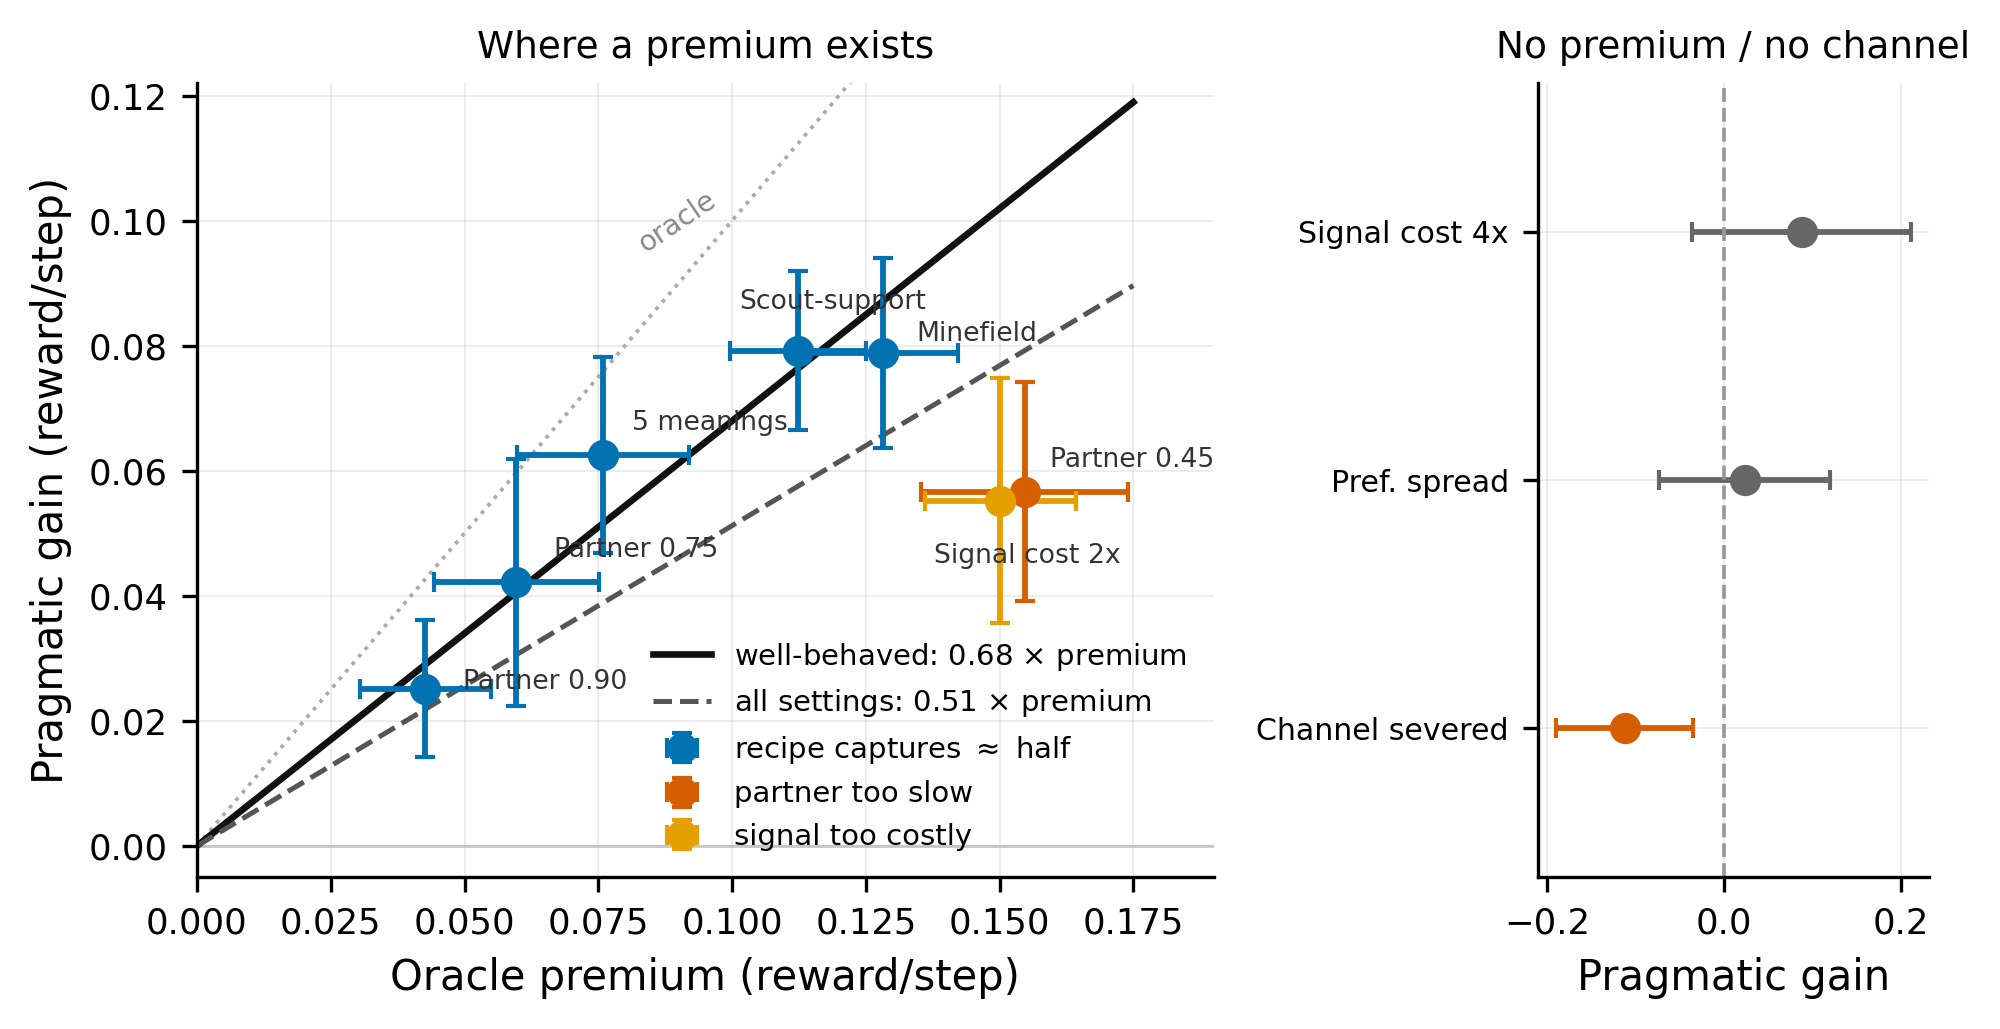
\includegraphics[width=0.90\columnwidth]{img/boundary_map.png}
\caption{The boundary map. \textbf{Left:} where the premium is resolvable, gain scales with it (solid: well-behaved fit $0.68\times$; dashed: all settings $0.51\times$; dotted: oracle); too-slow partners and too-costly signaling fall below despite large premiums. \textbf{Right:} no premium / no channel. Left bars $\pm1$ s.e.m., right bars $95\%$ CIs.}
\label{fig:boundary}
\end{figure}

\begin{figure}[htbp]
\centering
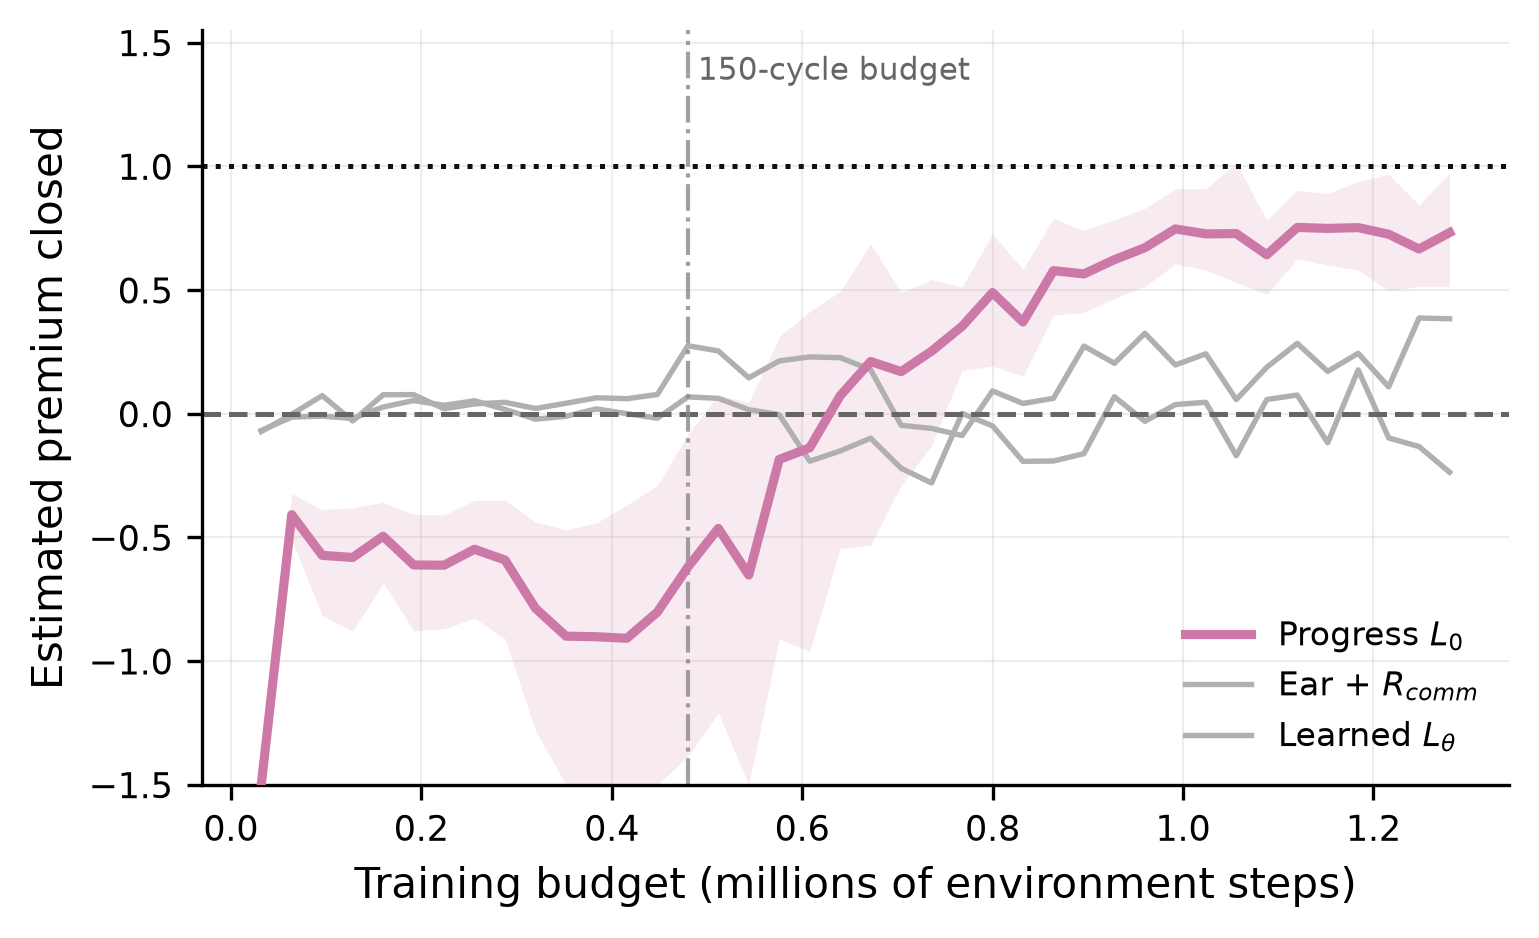
\includegraphics[width=0.84\columnwidth]{img/budget_dynamics.png}
\caption{The pre-convergence hazard: estimated fraction of the premium closed vs.\ the training budget at which the comparison is made (bootstrap $95\%$ bands, 10 seeds). The ordering stabilizes only past ${\sim}1$M steps.}
\label{fig:budget}
\end{figure}

\begin{figure}[htbp]
\centering
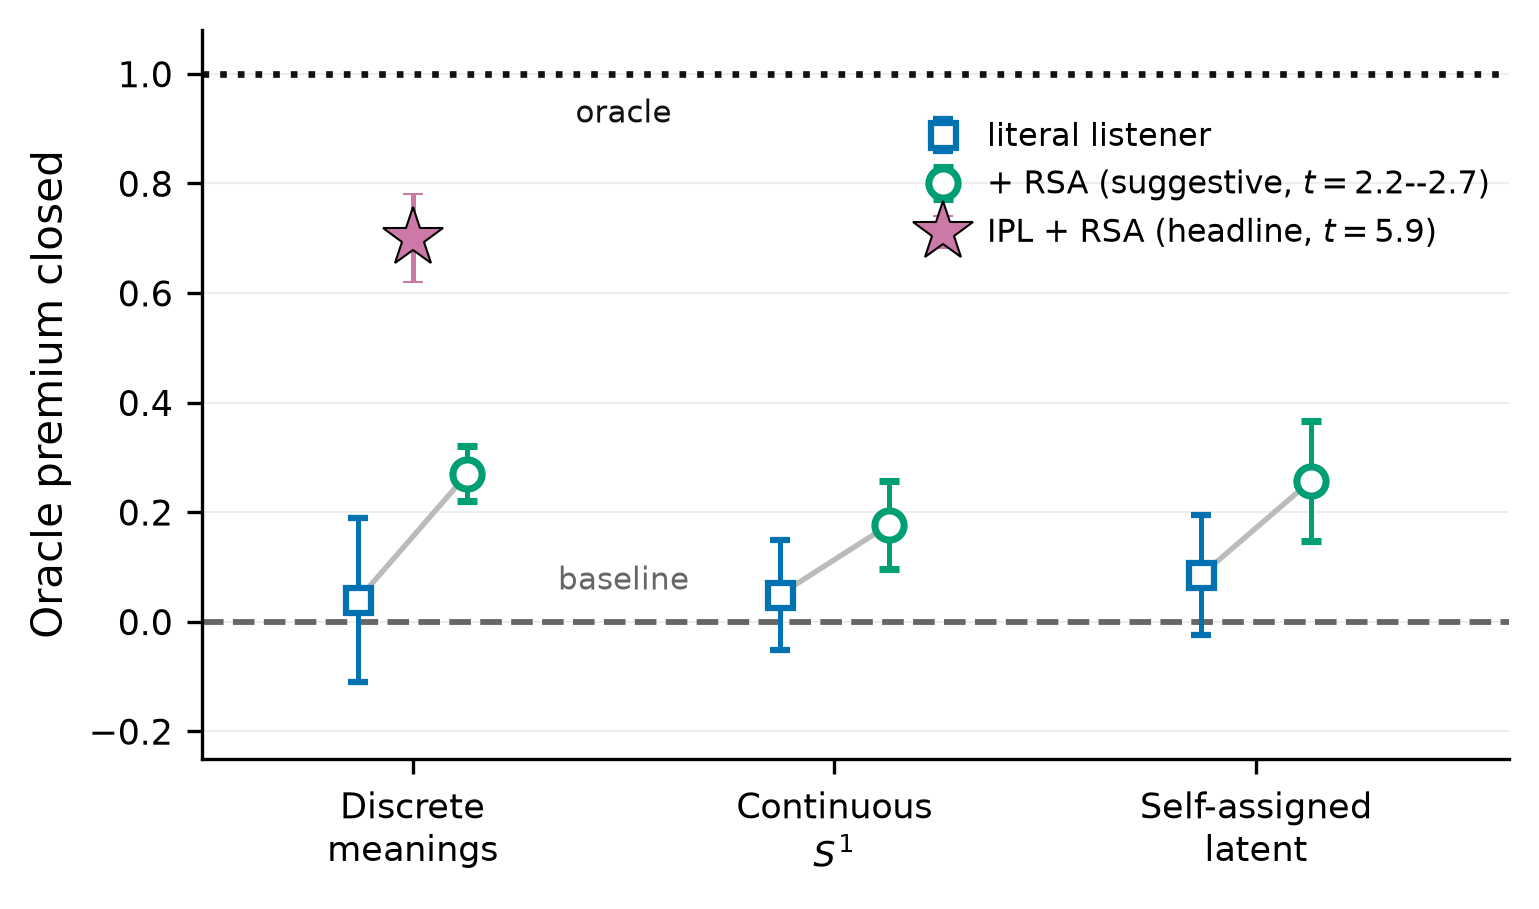
\includegraphics[width=0.94\columnwidth]{img/meaning_axis.png}
\caption{The meaning-space axis. In each regime the \emph{learned} listener without recursion sits near baseline and one RSA step lifts it by a similar fraction, but only the inverse-planning listener in the discrete regime clears the $t{\ge}4$ bar (filled star). Hand-crafted listeners (Table~\ref{tab:scout}, $60$--$82\%$) are a separate family, omitted to isolate the recursion's effect. Whiskers $\pm1$ s.e.m.\ as a fraction of each regime's oracle premium.}
\label{fig:meaning_axis}
\end{figure}

\begin{figure}[htbp]
\centering
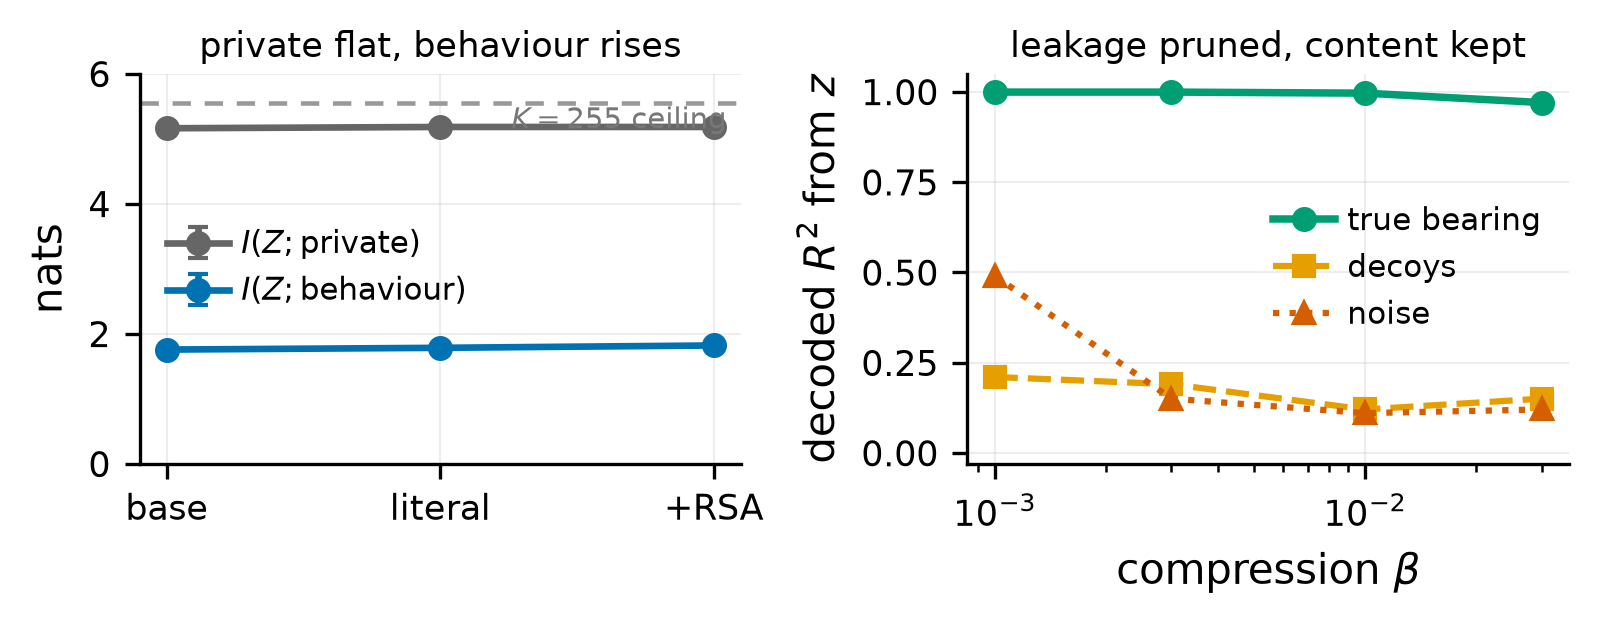
\includegraphics[width=\columnwidth]{img/transparency.png}
\caption{Compression chooses \emph{what} the latent carries: raising $\beta$ prunes decoded noise leakage and the decoys stay low, while the decision-relevant bearing remains fully decodable. The readability gap the pragmatic reward opens persists at every $\beta$.}
\label{fig:transparency}
\end{figure}

\section{Hyperparameters and Reproducibility}
\label{app:hyper}

\begin{table}[htbp]
\centering
\caption{Hyperparameters (all conditions unless noted).}
\label{tab:hyperparams}
\small
\setlength{\tabcolsep}{4pt}
\begin{tabular}{@{}>{\raggedright\arraybackslash}p{0.62\columnwidth}l@{}}
\toprule
\textbf{Parameter} & \textbf{Value} \\
\midrule
Parallel environments / episode length & 64 / 50 \\
Training cycles (both envs.; Env.\ B $\lambda$-sweep) & 400 (150) \\
Actor / critic architecture & MLP $256\times256$ \\
Learning rate (actor, critic) / listener & $3{\times}10^{-4}$ / $10^{-3}$ \\
Discount / target smoothing & 0.95 / 0.005 \\
Batch / updates per env step & 512 / 4 \\
Entropy target & $-\dim(\mathcal{A})$ (auto) \\
Listener $\Ltheta$ & MLP $128\times128$ \\
Direction listener temp.\ / $K$ / $N_r$ & 5 / 64 / 1 \\
Learned$+$RSA alternatives / $N_r$ & 16 / 1 \\
IPL tolerance $\kappa$ / alternatives / $N_r$ & 0.5 / 16 / 1 \\
Filter temp.\ / forgetting $\rho$ & 2 / 0.9 \\
$\lambda$ (Env.\ B / Env.\ A) / VOI weight & 0.1 / 0.3 / 0.2 \\
Scout / supporter speed; hist.\ window & 1.0 / 0.6; 6 \\
Bonus / cover / pickup radius & 3.0 / 0.3 / 0.3 \\
Integration step / damping / accel.\ gain & 0.1 / 0.25 / 5.0 \\
Arena clamp / site jitter / waypoint jitter & $\pm1.5$ / 0.1 / $\pm0.25$ \\
Mine penalty; replay; warm-up & 1.5; 400k; 2000 \\
Evaluation & every 10 cyc.\ (64 eps.) \\
\bottomrule
\end{tabular}
\end{table}

All environments, training, aggregation, and figure code will be released, with launch specifications determining every Environment A run exactly (JSON specs including seeds) and the Environment B command line documented in the repository README. One disclosed bug: an earlier snapshot evaluated the bounded-listener ear condition without the posterior injection it was trained with, producing an artifactual $0.551$ that persists in the archived histories; the corrected evaluation ($0.841\pm.023$), reproducible from the released checkpoints via the included re-evaluation script, is what we report.

\section{Environment B Details}
\label{app:envb}

Three agents and three colored landmarks in a continuous arena; each agent holds a private color preference; the team is rewarded for matched coverage, penalized for distance and collisions. Meanings are the three colors; every agent receives $\Rcomm$ under its own listener; $\lambda=0.1$.

\textbf{The weight $\lambda$ (exploratory, 150 cycles, 2 seeds/point).} With the learned listener, $\lambda$ behaves like a dial along an information--performance frontier, up to genuinely positive information gain at a large task cost at $\lambda=1$; with the exclusivity listener no operating point buys information---the reward is ignored at small $\lambda$ and destructive at moderate $\lambda$. Calibration is what turns $\lambda$ from a landmine into a dial.

\end{document}
